\documentclass{article}
\usepackage{textcomp}
\usepackage{fontenc}
\usepackage{graphicx}
\usepackage{caption}
\usepackage{gensymb} % for \degree
\usepackage{placeins} % for \images
\usepackage[margin=1in]{geometry} % to set margins
%\usepackage{cite} % for bibtex
\usepackage{natbib}

% \renewcommand{\familydefault}{\sfdefault}
\graphicspath{{images/}}	% Root directory of the figures
\setlength{\parskip}{2 mm}

% See IMPT NOTE re PNG figures! Below.

\usepackage{Sweave}
\begin{document}

 % 

\begin{center}
\textbf{\Large{Supporting Information \vspace{1ex}\\Temperature and photoperiod drive spring phenology across all species in a temperate forest community}}

Flynn \& Wolkovich
\end{center}

%% Add S prefix for tables and figures in Supplemental Materials
\renewcommand{\thetable}{S\arabic{table}}
\renewcommand{\thefigure}{S\arabic{figure}}

%%%%%%%%%%%%%%%%%%%%%%%%%%%%%%%
\section*{Supplemental Methods}
%%%%%%%%%%%%%%%%%%%%%%%%%%%%%%%

\noindent\emph{Temperature and photoperiod variation at study sites}

\noindent Spring climate regimes between our two sites (Harvard Forest and St. Hippolyte) vary, with temperatures generally being colder in the spring at the further north site (St. Hippolyte). Considering daily temperature data between 2000-2015 at both sites, daily minima, averaged over January-March each year, span -11.96 to -4.07\degree C and -19.74 to -8.88\degree C; daily maxima over the same period span -1.53 to 6.13\degree C and -9.99 to -0.26\degree C, at Harvard Forest and St. Hippolyte, respectively. Considering the period of April-May, daily minima span 2.90 to 6.19\degree C and 0.62 to 4.14\degree C; daily maxima over the same period span 14.23 to 19.00\degree C and 11.28 to 15.83\degree C at Harvard Forest and St. Hippolyte, respectively. 

\noindent As Saint Hippolyte is further north, its daylength (photoperiod) change in the spring is more extreme than at Harvard Forest: change from 1 March to 15 May is approximately 4 hours, while a similar change in Harvard Forest occurs over 1 March to 31 May. 

\noindent\emph{Chilling calculations}

\noindent The cuttings were harvested in late January 2015, and thus experienced substantial natural chilling by the time they were harvested. Using weather station data from the Harvard Forest and St. Hippolyte site, chilling hours (below 7.2\degree C), Utah Model chill portions \citep{utahmodel}, and Dynamic Model \citep{Erez:1988} chill portions were calculated both for the natural chilling experienced by harvest and the chilling experienced in the 4\degree C and 1.5\degree C treatments. 

\noindent The Utah Model and Dynamic Model of chill portions account for variation in the amount of chilling accumulated at different temperatures, with the greatest chilling occurring approximately between 5-10\degree C, and fewer chill portions accumulating at very low temperatures, and that higher temperatures can reduce accumulated chilling effects. The two differ in the parameters used to determine the shape of the chilling accumulation curve, with the Dynamic Model being shown to be the most successful in predicting phenology for some woody species \citep{Luedeling:2009}. With both the Utah and Dynamic Model, the more severe chilling treatment resulted in fewer calculated chilling portions (Table S7). 

\noindent To provide a comparison with estimated chilling under natural conditions we also show chilling for the study winter (2014-2015) until 1 April and 1 May (Table S7). Under the chilling hours and Utah model the greatest chilling occurred in our 4\degree C treatment, and both the 4\degree C and 1.5\degree C treatments provided more chilling than under natural conditions (until either 1 April or 1 May). In the Dynamic Model (chill portions) chilling was slightly higher by 1 May compared to our experimental chilling, but not when compared to 1 April. Taken together, our calculated chilling effects (Table S7) suggest that our experimental chilling effects would most likely have resulted in more chilling than experienced at either field site under natural conditions. 

\noindent\emph{Budburst and leafout success}

\noindent We assessed how species and treatments affected budburst and leafout success (Table S2) using a similar Bayesian hierarchical model as presented for days to budburst or leafout in the main text, but modeling species as a group only on the intercept (Fig. S2-S3) due to a limited amount of data (i.e., of all cuttings only 9.8-20.2\% did not burst bud or leaf out, yielding limited data when compared to days to budburst or leafout where we had continuous data for 79.8-90.2\% of all cuttings). Analysis of non-leafouts considered only the cuttings that burst bud (\emph{n}=1 926, rather than the total cutting number of \emph{n}=2 136). Models were fit in \verb|rstan| implemented via  \verb|rstanarm| version 2.17.2 using a binomial family and logit-link function. Full results are presented in Tables S3-S4 and Figures S2-S3.

\noindent Variation in budburst and leafout success was highest due to species identity and ranged from complete budburst and leafout (e.g., \emph{Hamamaelis}) to only 65\% budburst (\emph{Quercus alba}), 50\% or lower leafout (\emph{Fagus grandifolia}, \emph{Acer saccharum}, \emph{Kalmia angustifolia}) across all treatments (Table S2). The percent of non-leafouts by site was similar, with 20.6\% of Harvard Forest and 19.7\% of St. Hippolyte samples failing to leafout. Additional chilling decreased budburst and leafout success (Tables S3-S4; Fig. S2-S3), with 30 d at 1.5\degree C having the largest effects (cuttings with 1.5\degree C were 14.2\% less likely to reach budburst). Other effects were weaker and varied by budburst versus leafout (Tables S3-S4; Fig. S2-S3): for example, forcing temperatures and photoperiod affected leafout only (increased forcing increased leafout by 3.9\% while longer days increased leafout by 4.2\% though the combined effect of increased forcing and longer days together was only 3.0\% due to a negative interaction of the two effects, see Figure S3).

\noindent Days to budburst and days to leafout models performed on a subset of the data with higher rates of budburst (93\% overall) and leafout (88\%) produced qualitatively similar estimates, with most parameter estimates differing by less than 10\% compared to the full model. These models excluded the five species (\emph{Acer saccharum}, \emph{Fagus grandifolia}, \emph{Kalmia angustifolia}, \emph{Quercus alba} and \emph{Viburnum lantanoides}) that had budburst success below 80\% and/or leafout success below 75\%.

\noindent\emph{Effects of chilling at 16 and 32 days}

\noindent In the winter of 2015-2016 we conducted a follow-up study to test (1) whether our findings regarding different chilling temperatures in the winter of 2014-2015 were consistent across years and, (2) to test effects of chilling under a shorter duration of experimental chilling. For this experiment we tested the effects of field chilling plus chilling at two different temperatures, 1\degree C and 4 \degree C, and three different periods of chilling: no additional, 16 days or 32 days. Treatments were fully crossed resulting in six different combinations of treatment conditions. We collected cuttings as previously described from Harvard Forest on 18 December 2015 for seven species (\emph{Acer saccharum, Betula alleghaniensis, Fagus grandifolia, Hamamelis virginiana, Ilex mucronatus, Quercus rubra, Viburnum cassinoides}). All cuttings were kept at 4\degree C until 1 January when they were put into treatment conditions. Forcing conditions were set as 20\degree C days with 10\degree C nights and 12 hour photoperiods. We assessed how species and treatments affected days to budburst using a similar Bayesian hierarchical model as presented for days to budburst or leafout in the main text but for this set of treatments (models were fit in \verb|rstan| implemented via  \verb|rstanarm| version 2.17.2). 

\noindent Our findings were generally consistent with those from our previous year's experiment: effects of chilling were similar across the two temperatures (1\degree C and 4\degree C, Figure S9). Additional chilling time advanced budburst by 7.8 or 10.4 days, for 16 or 32 additional days of chilling, respectively (Fig. S9). The additional advance of only 2.6 days between the treatments of 16 and 32 days experimental chilling suggests that effects of chilling over time are non-linear and that additional chilling time beyond 32 days may have had only small effects, this is consistent with metrics of chilling units (see Table S7), which suggests our previous year's experimental chilling would have been as high (or higher) than a full season of field chilling. 

% see budchill/analyses/budchill_analysis.R 

% http://andrewgelman.com/2016/11/05/why-i-prefer-50-to-95-intervals/

%%%%%%%%%%%%%%%%%%%%%%%%%%%%%%%%%%%%
% \subsection*{References Cited}
%%%%%%%%%%%%%%%%%%%%%%%%%%%%%%%%%%%%

\bibliography{danlib}
\bibliographystyle{newphyto}

\newpage
%%%%%%%%%%%%%%%%%%%%%%%%%%%%%%%
\section*{Supplemental Figures and Tables}
%%%%%%%%%%%%%%%%%%%%%%%%%%%%%%%


% latex table generated in R 3.3.3 by xtable 1.8-2 package
% Fri Mar 16 13:10:03 2018
\begin{table}[ht]
\centering
\caption{Mean leafout and budburst days after exposure to controlled environment forcing conditions (across all treatments, based on raw data) for the 28 species at both Harvard Forest (HF), USA and St. Hippoltye (SH), Canada.} 
\begin{tabular}{lrrrr}
  \hline
Species & Budburst.HF & Budburst.SH & Leafout.HF & Leafout.SH \\ 
  \hline
\textit{Acer pensylvanicum} & 16.40 & 18.33 & 40.88 & 46.94 \\ 
  \textit{Acer rubrum} & 22.40 & 25.15 & 40.59 & 44.40 \\ 
  \textit{Acer saccharum} & 44.96 & 36.48 & 57.07 & 46.88 \\ 
  \textit{Alnus incana subsp. rugosa} & 32.91 & 25.36 & 45.15 & 44.36 \\ 
  \textit{Aronia melanocarpa} & 13.62 &  & 29.83 &  \\ 
  \textit{Betula alleghaniensis} & 19.67 & 20.77 & 33.51 & 34.64 \\ 
  \textit{Betula lenta} & 29.83 &  & 50.57 &  \\ 
  \textit{Betula papyrifera} & 16.89 & 18.04 & 28.71 & 35.63 \\ 
  \textit{Corylus cornuta} & 24.86 & 19.04 & 33.95 & 30.38 \\ 
  \textit{Fagus grandifolia} & 41.82 & 43.13 & 48.54 & 46.90 \\ 
  \textit{Fraxinus nigra} & 38.00 & 38.00 & 52.28 & 46.91 \\ 
  \textit{Hamamelis virginiana} & 43.67 &  & 47.38 &  \\ 
  \textit{Ilex mucronatus} & 15.80 & 15.49 & 26.97 & 25.15 \\ 
  \textit{Kalmia angustifolia} & 30.25 & 32.48 & 37.80 & 42.20 \\ 
  \textit{Lonicera canadensis} & 16.91 & 15.75 & 28.26 & 25.08 \\ 
  \textit{Lyonia ligustrina} & 30.87 &  & 49.50 &  \\ 
  \textit{Nyssa sylvatica} & 31.65 &  & 52.87 &  \\ 
  \textit{Populus grandidentata} & 33.43 & 31.23 & 46.21 & 45.17 \\ 
  \textit{Prunus pensylvanica} & 17.81 & 16.21 & 32.13 & 29.65 \\ 
  \textit{Quercus alba} & 45.23 &  & 52.91 &  \\ 
  \textit{Quercus rubra} & 36.43 & 33.57 & 45.02 & 42.80 \\ 
  \textit{Quercus velutina} & 52.09 &  & 59.16 &  \\ 
  \textit{Rhamnus frangula} & 32.38 &  & 37.29 &  \\ 
  \textit{Rhododendron prinophyllum} & 29.25 &  & 52.14 &  \\ 
  \textit{Spiraea alba} & 18.00 & 20.21 & 25.94 & 24.62 \\ 
  \textit{Vaccinium myrtilloides} & 13.12 & 17.27 & 27.00 & 28.95 \\ 
  \textit{Viburnum cassinoides} & 15.41 & 18.46 & 16.80 & 18.71 \\ 
  \textit{Viburnum lantanoides} & 31.25 & 27.54 & 32.02 & 26.41 \\ 
   \hline
\end{tabular}
\end{table}
% latex table generated in R 3.3.3 by xtable 1.8-2 package
% Fri Mar 16 13:10:03 2018
\begin{table}[ht]
\centering
\caption{Mean leafout and budburst success after exposure to controlled environment forcing conditions (across all treatments, based on raw data) for the 28 species.} 
\begin{tabular}{lrr}
  \hline
Species & Budburst.success & Leafout.success \\ 
  \hline
\textit{Acer pensylvanicum} & 0.99 & 0.78 \\ 
  \textit{Acer rubrum} & 0.92 & 0.79 \\ 
  \textit{Acer saccharum} & 0.78 & 0.47 \\ 
  \textit{Alnus incana subsp. rugosa} & 0.94 & 0.88 \\ 
  \textit{Aronia melanocarpa} & 0.81 & 0.75 \\ 
  \textit{Betula alleghaniensis} & 0.97 & 0.95 \\ 
  \textit{Betula lenta} & 1.00 & 0.96 \\ 
  \textit{Betula papyrifera} & 0.93 & 0.92 \\ 
  \textit{Corylus cornuta} & 0.94 & 0.92 \\ 
  \textit{Fagus grandifolia} & 0.80 & 0.49 \\ 
  \textit{Fraxinus nigra} & 0.88 & 0.85 \\ 
  \textit{Hamamelis virginiana} & 1.00 & 1.00 \\ 
  \textit{Ilex mucronatus} & 0.97 & 0.97 \\ 
  \textit{Kalmia angustifolia} & 0.98 & 0.21 \\ 
  \textit{Lonicera canadensis} & 0.97 & 0.97 \\ 
  \textit{Lyonia ligustrina} & 0.96 & 0.92 \\ 
  \textit{Nyssa sylvatica} & 0.96 & 0.96 \\ 
  \textit{Populus grandidentata} & 0.83 & 0.77 \\ 
  \textit{Prunus pensylvanica} & 0.89 & 0.84 \\ 
  \textit{Quercus alba} & 0.65 & 0.55 \\ 
  \textit{Quercus rubra} & 0.95 & 0.91 \\ 
  \textit{Quercus velutina} & 0.92 & 0.79 \\ 
  \textit{Rhamnus frangula} & 1.00 & 0.88 \\ 
  \textit{Rhododendron prinophyllum} & 1.00 & 0.92 \\ 
  \textit{Spiraea alba} & 0.80 & 0.78 \\ 
  \textit{Vaccinium myrtilloides} & 0.96 & 0.94 \\ 
  \textit{Viburnum cassinoides} & 0.89 & 0.89 \\ 
  \textit{Viburnum lantanoides} & 0.79 & 0.75 \\ 
   \hline
\end{tabular}
\end{table}

\clearpage
\newpage

% latex table generated in R 3.3.3 by xtable 1.8-2 package
% Fri Mar 16 13:10:03 2018
\begin{table}[ht]
\centering
\caption{Summary of mixed-effects model of budburst success (estimates presented on logit scale). See also Figure S2.} 
\begin{tabular}{rrrrrrr}
  \hline
 & mean & sd & 2.5\% & 50\% & 97.5\% & Rhat \\ 
  \hline
Forcing Temperature & -0.09 & 0.31 & -0.71 & -0.09 & 0.51 & 1.00 \\ 
  Photoperiod & -0.01 & 0.31 & -0.61 & -0.01 & 0.62 & 1.00 \\ 
  Chilling 4 \degree C & -0.70 & 0.40 & -1.47 & -0.71 & 0.10 & 1.00 \\ 
  Chilling 1.5 \degree C & -1.48 & 0.35 & -2.17 & -1.48 & -0.80 & 1.00 \\ 
  Site & 0.42 & 0.35 & -0.24 & 0.41 & 1.12 & 1.00 \\ 
  Forcing Temperature $\times$ Photoperiod & -0.31 & 0.31 & -0.94 & -0.31 & 0.30 & 1.00 \\ 
  Forcing Temperature $\times$ Chilling 4 \degree C & 0.59 & 0.41 & -0.21 & 0.59 & 1.38 & 1.00 \\ 
  Forcing Temperature $\times$ Chilling 1.5 \degree C & 0.02 & 0.35 & -0.65 & 0.03 & 0.70 & 1.00 \\ 
  Photoperiod $\times$ Chilling 4 \degree C & 0.58 & 0.42 & -0.24 & 0.58 & 1.37 & 1.00 \\ 
  Photoperiod $\times$ Chilling 1.5 \degree C & 0.48 & 0.34 & -0.19 & 0.48 & 1.15 & 1.00 \\ 
  Forcing Temperature $\times$ Site & -0.22 & 0.31 & -0.82 & -0.22 & 0.39 & 1.00 \\ 
  Photoperiod $\times$ Site & -0.07 & 0.31 & -0.68 & -0.07 & 0.52 & 1.00 \\ 
  Site $\times$ Chilling 4 \degree C & 0.15 & 0.42 & -0.66 & 0.14 & 0.97 & 1.00 \\ 
  Site $\times$ Chilling 1.5 \degree C & 0.50 & 0.36 & -0.21 & 0.50 & 1.18 & 1.00 \\ 
   \hline
\end{tabular}
\end{table}
% latex table generated in R 3.3.3 by xtable 1.8-2 package
% Fri Mar 16 13:10:03 2018
\begin{table}[ht]
\centering
\caption{Summary of mixed-effects model of leafout success (estimates presented on logit scale). See also Figure S3.} 
\begin{tabular}{rrrrrrr}
  \hline
 & mean & sd & 2.5\% & 50\% & 97.5\% & Rhat \\ 
  \hline
Forcing Temperature & 1.09 & 0.35 & 0.39 & 1.08 & 1.80 & 1.00 \\ 
  Photoperiod & 1.27 & 0.35 & 0.59 & 1.27 & 1.96 & 1.00 \\ 
  Chilling 4 \degree C & -0.84 & 0.41 & -1.63 & -0.85 & -0.04 & 1.00 \\ 
  Chilling 1.5 \degree C & -1.88 & 0.40 & -2.63 & -1.88 & -1.10 & 1.00 \\ 
  Site & -0.29 & 0.35 & -0.98 & -0.29 & 0.37 & 1.00 \\ 
  Forcing Temperature $\times$ Photoperiod & -1.64 & 0.35 & -2.30 & -1.63 & -0.95 & 1.00 \\ 
  Forcing Temperature $\times$ Chilling 4 \degree C & 0.67 & 0.44 & -0.19 & 0.66 & 1.56 & 1.00 \\ 
  Forcing Temperature $\times$ Chilling 1.5 \degree C & 0.38 & 0.43 & -0.46 & 0.38 & 1.19 & 1.00 \\ 
  Photoperiod $\times$ Chilling 4 \degree C & 0.21 & 0.42 & -0.65 & 0.21 & 1.04 & 1.00 \\ 
  Photoperiod $\times$ Chilling 1.5 \degree C & 0.54 & 0.41 & -0.25 & 0.54 & 1.33 & 1.00 \\ 
  Forcing Temperature $\times$ Site & 0.24 & 0.36 & -0.49 & 0.24 & 0.94 & 1.00 \\ 
  Photoperiod $\times$ Site & -0.40 & 0.35 & -1.09 & -0.41 & 0.30 & 1.00 \\ 
  Site $\times$ Chilling 4 \degree C & 0.13 & 0.44 & -0.74 & 0.13 & 1.01 & 1.00 \\ 
  Site $\times$ Chilling 1.5 \degree C & 0.80 & 0.41 & -0.00 & 0.81 & 1.59 & 1.00 \\ 
   \hline
\end{tabular}
\end{table}

% latex table generated in R 3.3.3 by xtable 1.8-2 package
% Fri Mar 16 13:10:04 2018
\begin{table}[ht]
\centering
\caption{Summary of mixed-effects model of budburst day. See also Figure S4} 
\begin{tabular}{rrrrrrr}
  \hline
 & mean & sd & 2.5\% & 50\% & 97.5\% & Rhat \\ 
  \hline
Forcing Temperature & -8.82 & 1.05 & -10.87 & -8.82 & -6.73 & 1.00 \\ 
  Photoperiod & -4.53 & 0.90 & -6.28 & -4.53 & -2.73 & 1.00 \\ 
  Chilling 4 \degree C & -15.82 & 2.13 & -20.06 & -15.82 & -11.59 & 1.00 \\ 
  Chilling 1.5 \degree C & -13.13 & 2.00 & -17.04 & -13.14 & -9.08 & 1.00 \\ 
  Site & 1.31 & 1.08 & -0.84 & 1.31 & 3.45 & 1.00 \\ 
  Forcing Temperature $\times$ Photoperiod & -0.62 & 0.79 & -2.14 & -0.63 & 0.95 & 1.00 \\ 
  Forcing Temperature $\times$ Chilling 4 \degree C & 9.09 & 1.09 & 6.94 & 9.09 & 11.23 & 1.00 \\ 
  Forcing Temperature $\times$ Chilling 1.5 \degree C & 9.78 & 1.17 & 7.50 & 9.79 & 12.07 & 1.00 \\ 
  Photoperiod $\times$ Chilling 4 \degree C & -0.26 & 1.11 & -2.48 & -0.26 & 1.98 & 1.00 \\ 
  Photoperiod $\times$ Chilling 1.5 \degree C & -0.14 & 1.25 & -2.63 & -0.13 & 2.27 & 1.00 \\ 
  Forcing Temperature $\times$ Site & -1.51 & 0.85 & -3.13 & -1.51 & 0.16 & 1.00 \\ 
  Photoperiod $\times$ Site & -0.08 & 0.81 & -1.70 & -0.08 & 1.49 & 1.00 \\ 
  Site $\times$ Chilling 4 \degree C & -2.26 & 1.21 & -4.64 & -2.25 & 0.13 & 1.00 \\ 
  Site $\times$ Chilling 1.5 \degree C & -3.47 & 1.34 & -6.10 & -3.48 & -0.85 & 1.00 \\ 
   \hline
\end{tabular}
\end{table}
% latex table generated in R 3.3.3 by xtable 1.8-2 package
% Fri Mar 16 13:10:04 2018
\begin{table}[ht]
\centering
\caption{Summary of mixed-effects model of leafout day. See also Figure S5.} 
\begin{tabular}{rrrrrrr}
  \hline
 & mean & sd & 2.5\% & 50\% & 97.5\% & Rhat \\ 
  \hline
Forcing Temperature & -19.06 & 1.04 & -21.10 & -19.05 & -17.05 & 1.00 \\ 
  Photoperiod & -11.19 & 0.86 & -12.91 & -11.18 & -9.53 & 1.00 \\ 
  Chilling 4 \degree C & -17.44 & 2.07 & -21.55 & -17.42 & -13.34 & 1.00 \\ 
  Chilling 1.5 \degree C & -15.84 & 2.05 & -20.02 & -15.80 & -11.88 & 1.00 \\ 
  Site & 1.34 & 1.24 & -1.12 & 1.35 & 3.76 & 1.00 \\ 
  Forcing Temperature $\times$ Photoperiod & 3.68 & 0.85 & 2.06 & 3.66 & 5.39 & 1.00 \\ 
  Forcing Temperature $\times$ Chilling 4 \degree C & 10.30 & 1.17 & 8.01 & 10.30 & 12.62 & 1.00 \\ 
  Forcing Temperature $\times$ Chilling 1.5 \degree C & 11.22 & 1.32 & 8.61 & 11.24 & 13.81 & 1.00 \\ 
  Photoperiod $\times$ Chilling 4 \degree C & 0.79 & 1.18 & -1.47 & 0.79 & 3.16 & 1.00 \\ 
  Photoperiod $\times$ Chilling 1.5 \degree C & 2.35 & 1.32 & -0.32 & 2.37 & 4.87 & 1.00 \\ 
  Forcing Temperature $\times$ Site & -0.50 & 0.83 & -2.11 & -0.50 & 1.15 & 1.00 \\ 
  Photoperiod $\times$ Site & -0.87 & 0.83 & -2.51 & -0.87 & 0.75 & 1.00 \\ 
  Site $\times$ Chilling 4 \degree C & -1.75 & 1.28 & -4.26 & -1.76 & 0.77 & 1.00 \\ 
  Site $\times$ Chilling 1.5 \degree C & -3.35 & 1.51 & -6.35 & -3.34 & -0.41 & 1.00 \\ 
   \hline
\end{tabular}
\end{table}
\clearpage
\newpage

% latex table generated in R 3.3.3 by xtable 1.8-2 package
% Fri Mar 16 13:10:04 2018
\begin{table}[ht]
\centering
\caption{Chill units in the field before harvest (January 2015), until 1 April and 1 May 2015 at each site, and in growth chamber conditions (including field chilling experienced before cuttings entered the chambers).} 
\begin{tabular}{llrrr}
  \hline
Site & Treatment & Chilling Hours & Utah Model & Chill portions \\ 
  \hline
Harvard Forest & Field chilling until collection & 892 & 814.50 & 56.62 \\ 
   & Field chilling to 1 Apr & 1153 & 980.00 & 79.37 \\ 
   & Field chilling to 1 May & 1449 & 1360.50 & 99.94 \\ 
   & Field chilling + 4.0 \degree C x 30 d & 2140 & 2062.50 & 94.06 \\ 
   & Field chilling + 1.5 \degree C x 30 d & 2140 & 1702.50 & 91.17 \\ 
  St. Hippolyte & Field chilling until collection & 682 & 599.50 & 44.63 \\ 
   & Field chilling to 1 Apr & 796 & 653.50 & 63.55 \\ 
   & Field chilling to 1 May & 1166 & 937.00 & 83.83 \\ 
   & Field chilling + 4.0 \degree C x 30 d & 1930 & 1847.50 & 82.06 \\ 
   & Field chilling + 1.5 \degree C x 30 d & 1930 & 1487.50 & 79.18 \\ 
   \hline
\end{tabular}
\end{table}

%% \clearpage % use if get 'too many unprocessed floats' error

\clearpage 
% IMPT NOTE re PNG figures: Annoyingly, Sweave seems to delete the degree marks from the Advplot2 and 4 panel figs. They run fine if output from Pheno Budburst Analysis.R ... I could fix this I am sure, but for cheap sake, I just changed them to PNG. This is important to remember if the data or analysis ever changes!!

% Fig S1: Raw data plot

\begin{figure} 
\begin{center}
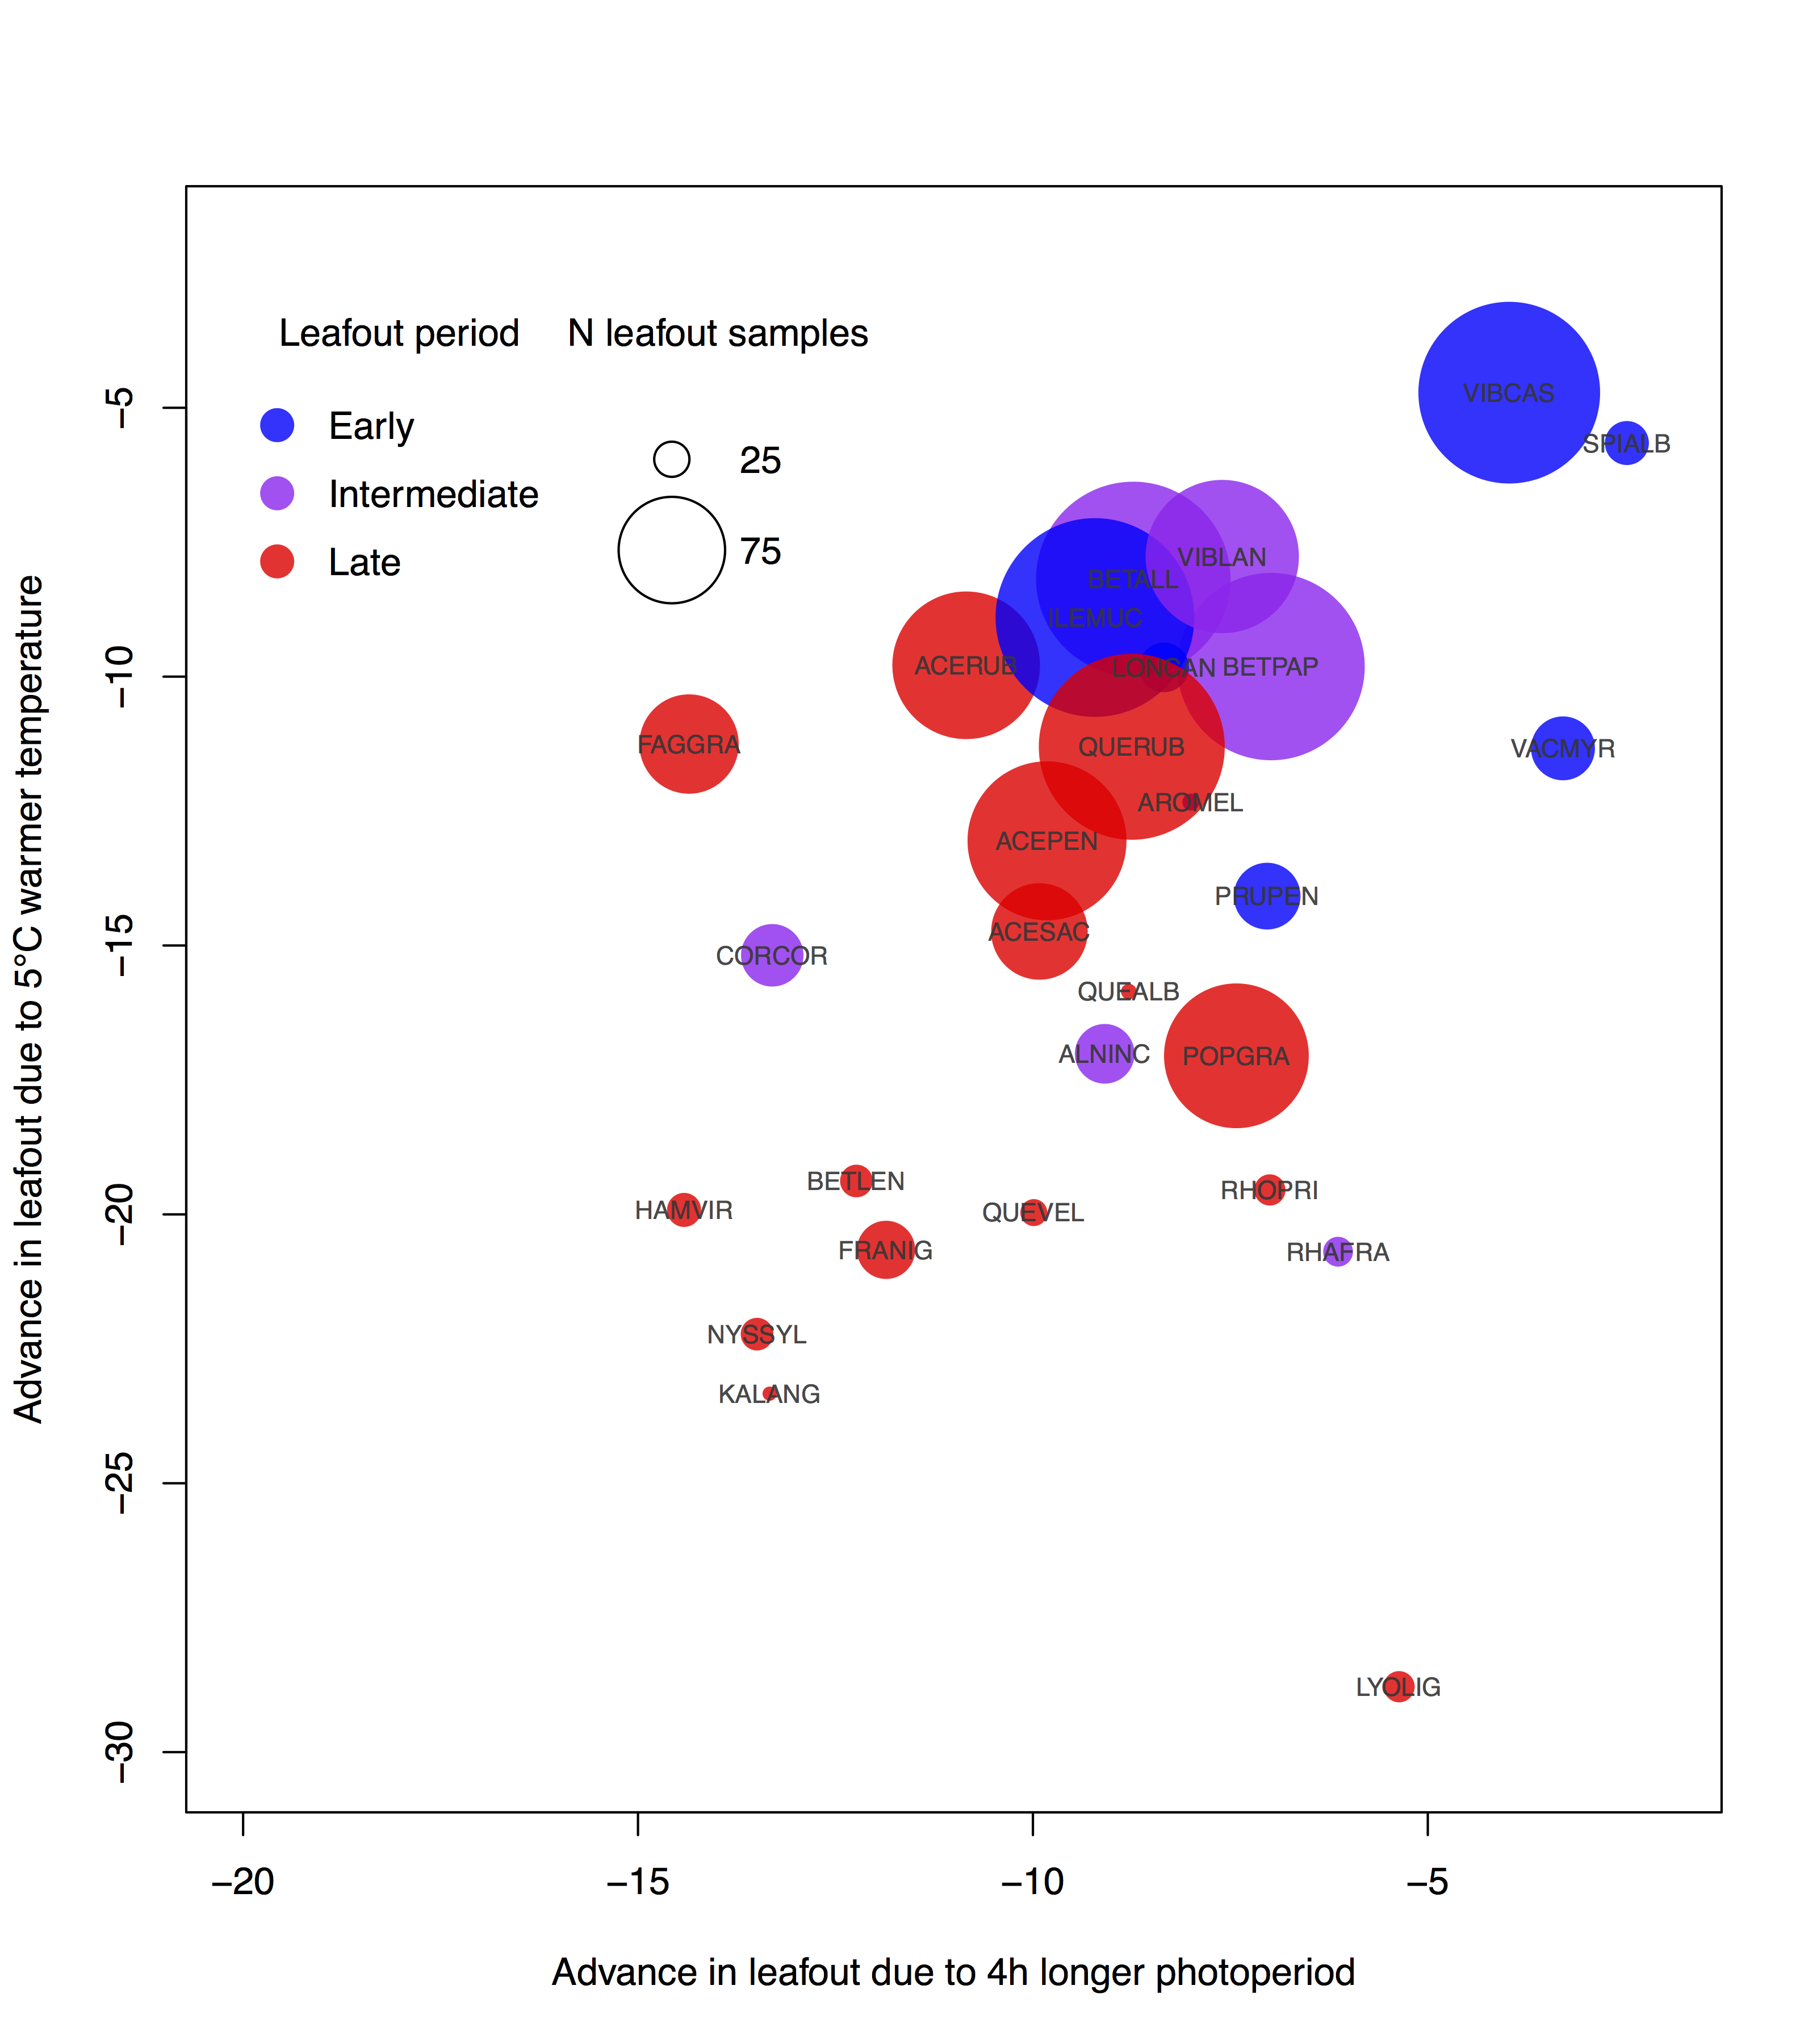
\includegraphics[scale=0.5]{Advplot2.png}
\caption{Responses of 28 woody plant species to photoperiod and temperature cues for leafout. Color of circle reflect unmodeled data on average leafout day across treatments, across sites of origin, while size of circle represents the total number of clippings in the experiment---this varies mainly based on whether the species was found at both sites and whether it was exposed to all three chilling treatments. } % Changed legend, check that I did it correctly please! Yes, ok.
\label{fig:fig1}
\end{center}
\end{figure}

\begin{figure}
\label{fig:figS8}
\includegraphics[width=1\textwidth, page=1]{NonBBLO_sp_m2} % built in Analyzing non-leafouts.R 
\caption{Model estimates of budburst success, including species-level effects, presented on logit scale. Dots and bars show mean and 50\% credible intervals. See also Table S3.}
\end{figure}

\begin{figure}
\label{fig:figS9}
\includegraphics[width=1\textwidth, page=2]{NonBBLO_sp_m2}
\caption{Model estimates of leafout success, including species-level effects, presented on logit scale. Dots and bars show mean and 50\% credible intervals. See also Table S4.}
\end{figure}

\begin{figure}
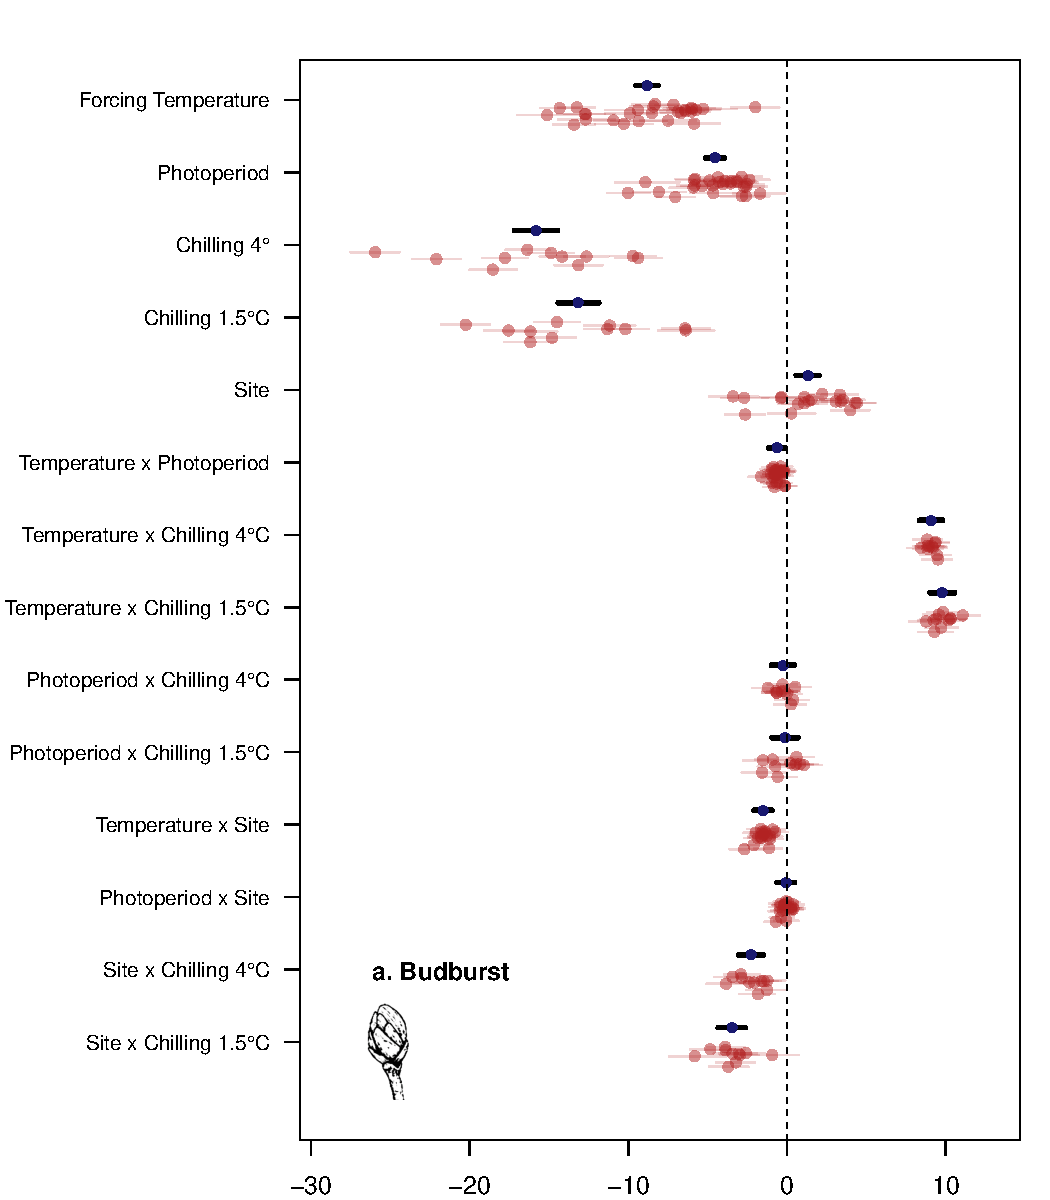
\includegraphics[width=1\textwidth, page=1]{Fig1_bb_lo+sp} % built in Additional Plots and Processing.R
\caption{Model estimates of effects of each predictor on budburst day, including species-level effects. Dots and bars show mean and 50\% credible intervals.}
\label{fig:figS2}
\end{figure}

\clearpage

\begin{figure}
\includegraphics[width=1\textwidth, page=2]{Fig1_bb_lo+sp}
\caption{Model estimates of leafout day, including species-level effects. Dots and bars show mean and 50\% credible intervals.}
\label{fig:figS3}
\end{figure}

\begin{figure}
\label{fig:figS5}
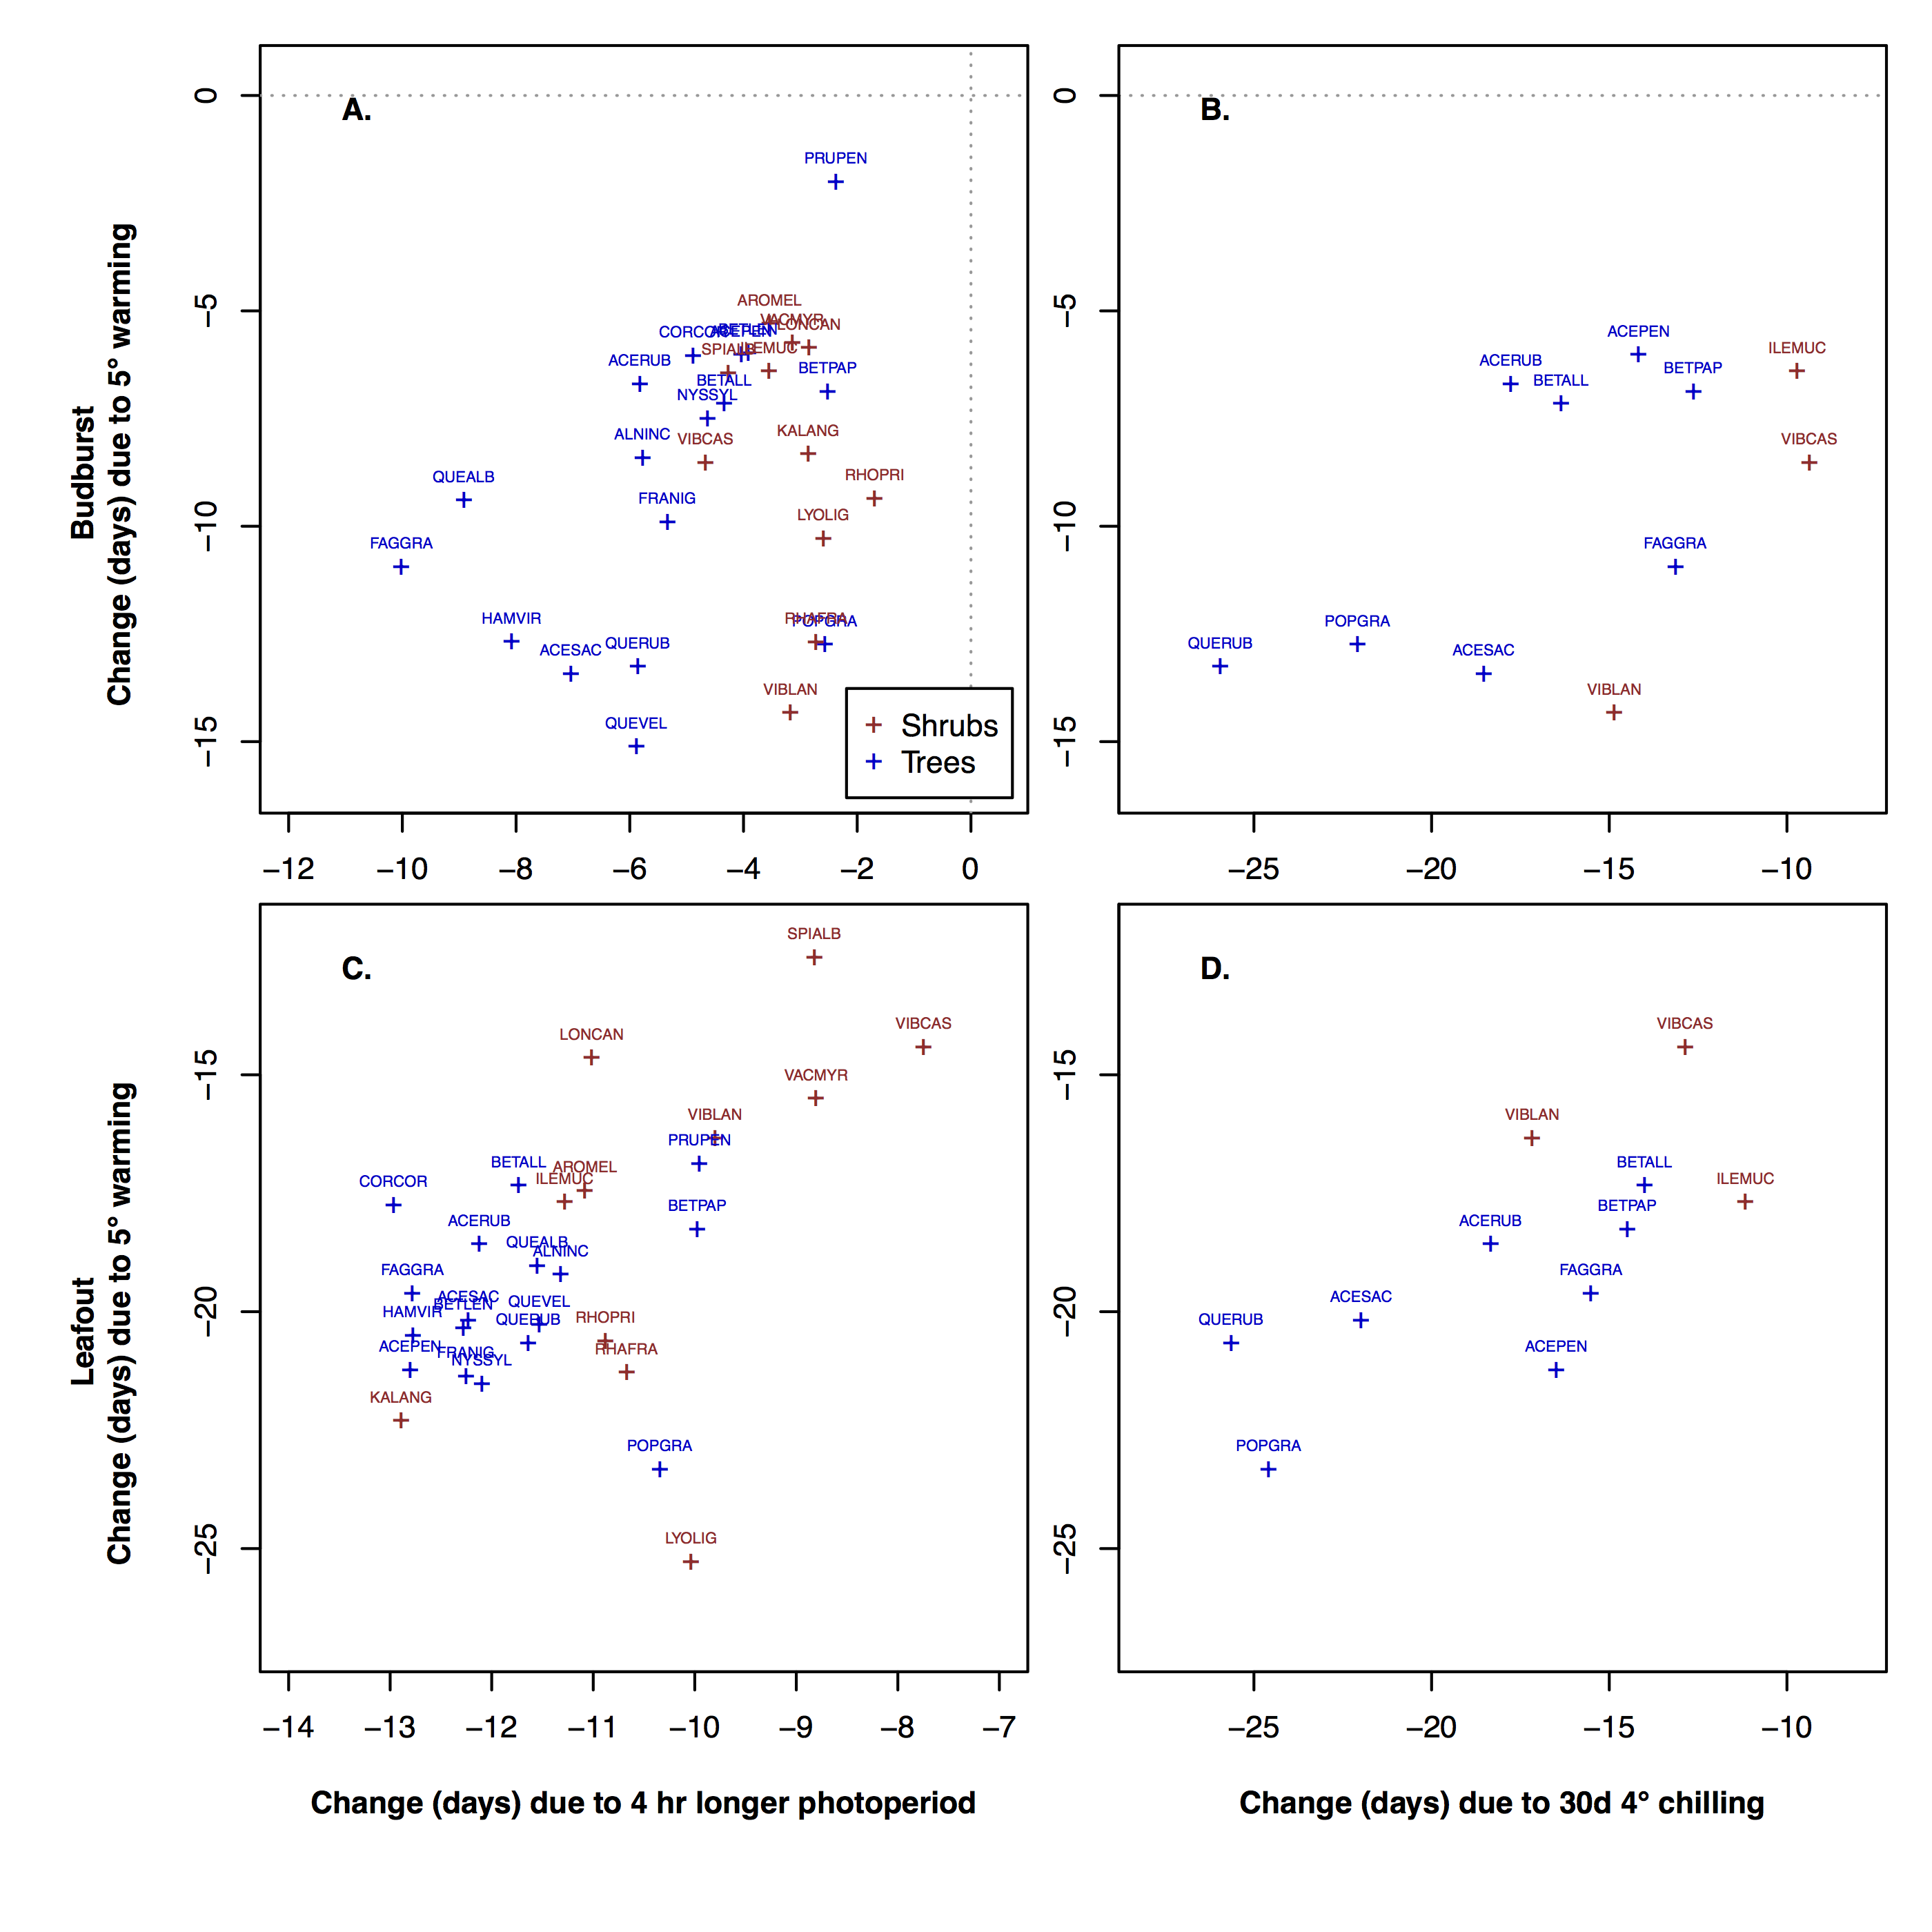
\includegraphics[width=1\textwidth]{Fig2_4panel_ZoomSupp.png}
\caption{Effects of photoperiod, temperature and chilling across species (shrub species shown in red, tree species in blue): Similar to Fig. 2 from main text, but designed to make species names easier to read by adjusting axes (note that axes vary across rows and columns) and removing bars showing credible intervals. }
\end{figure}


\begin{figure}
\label{fig:figS6}
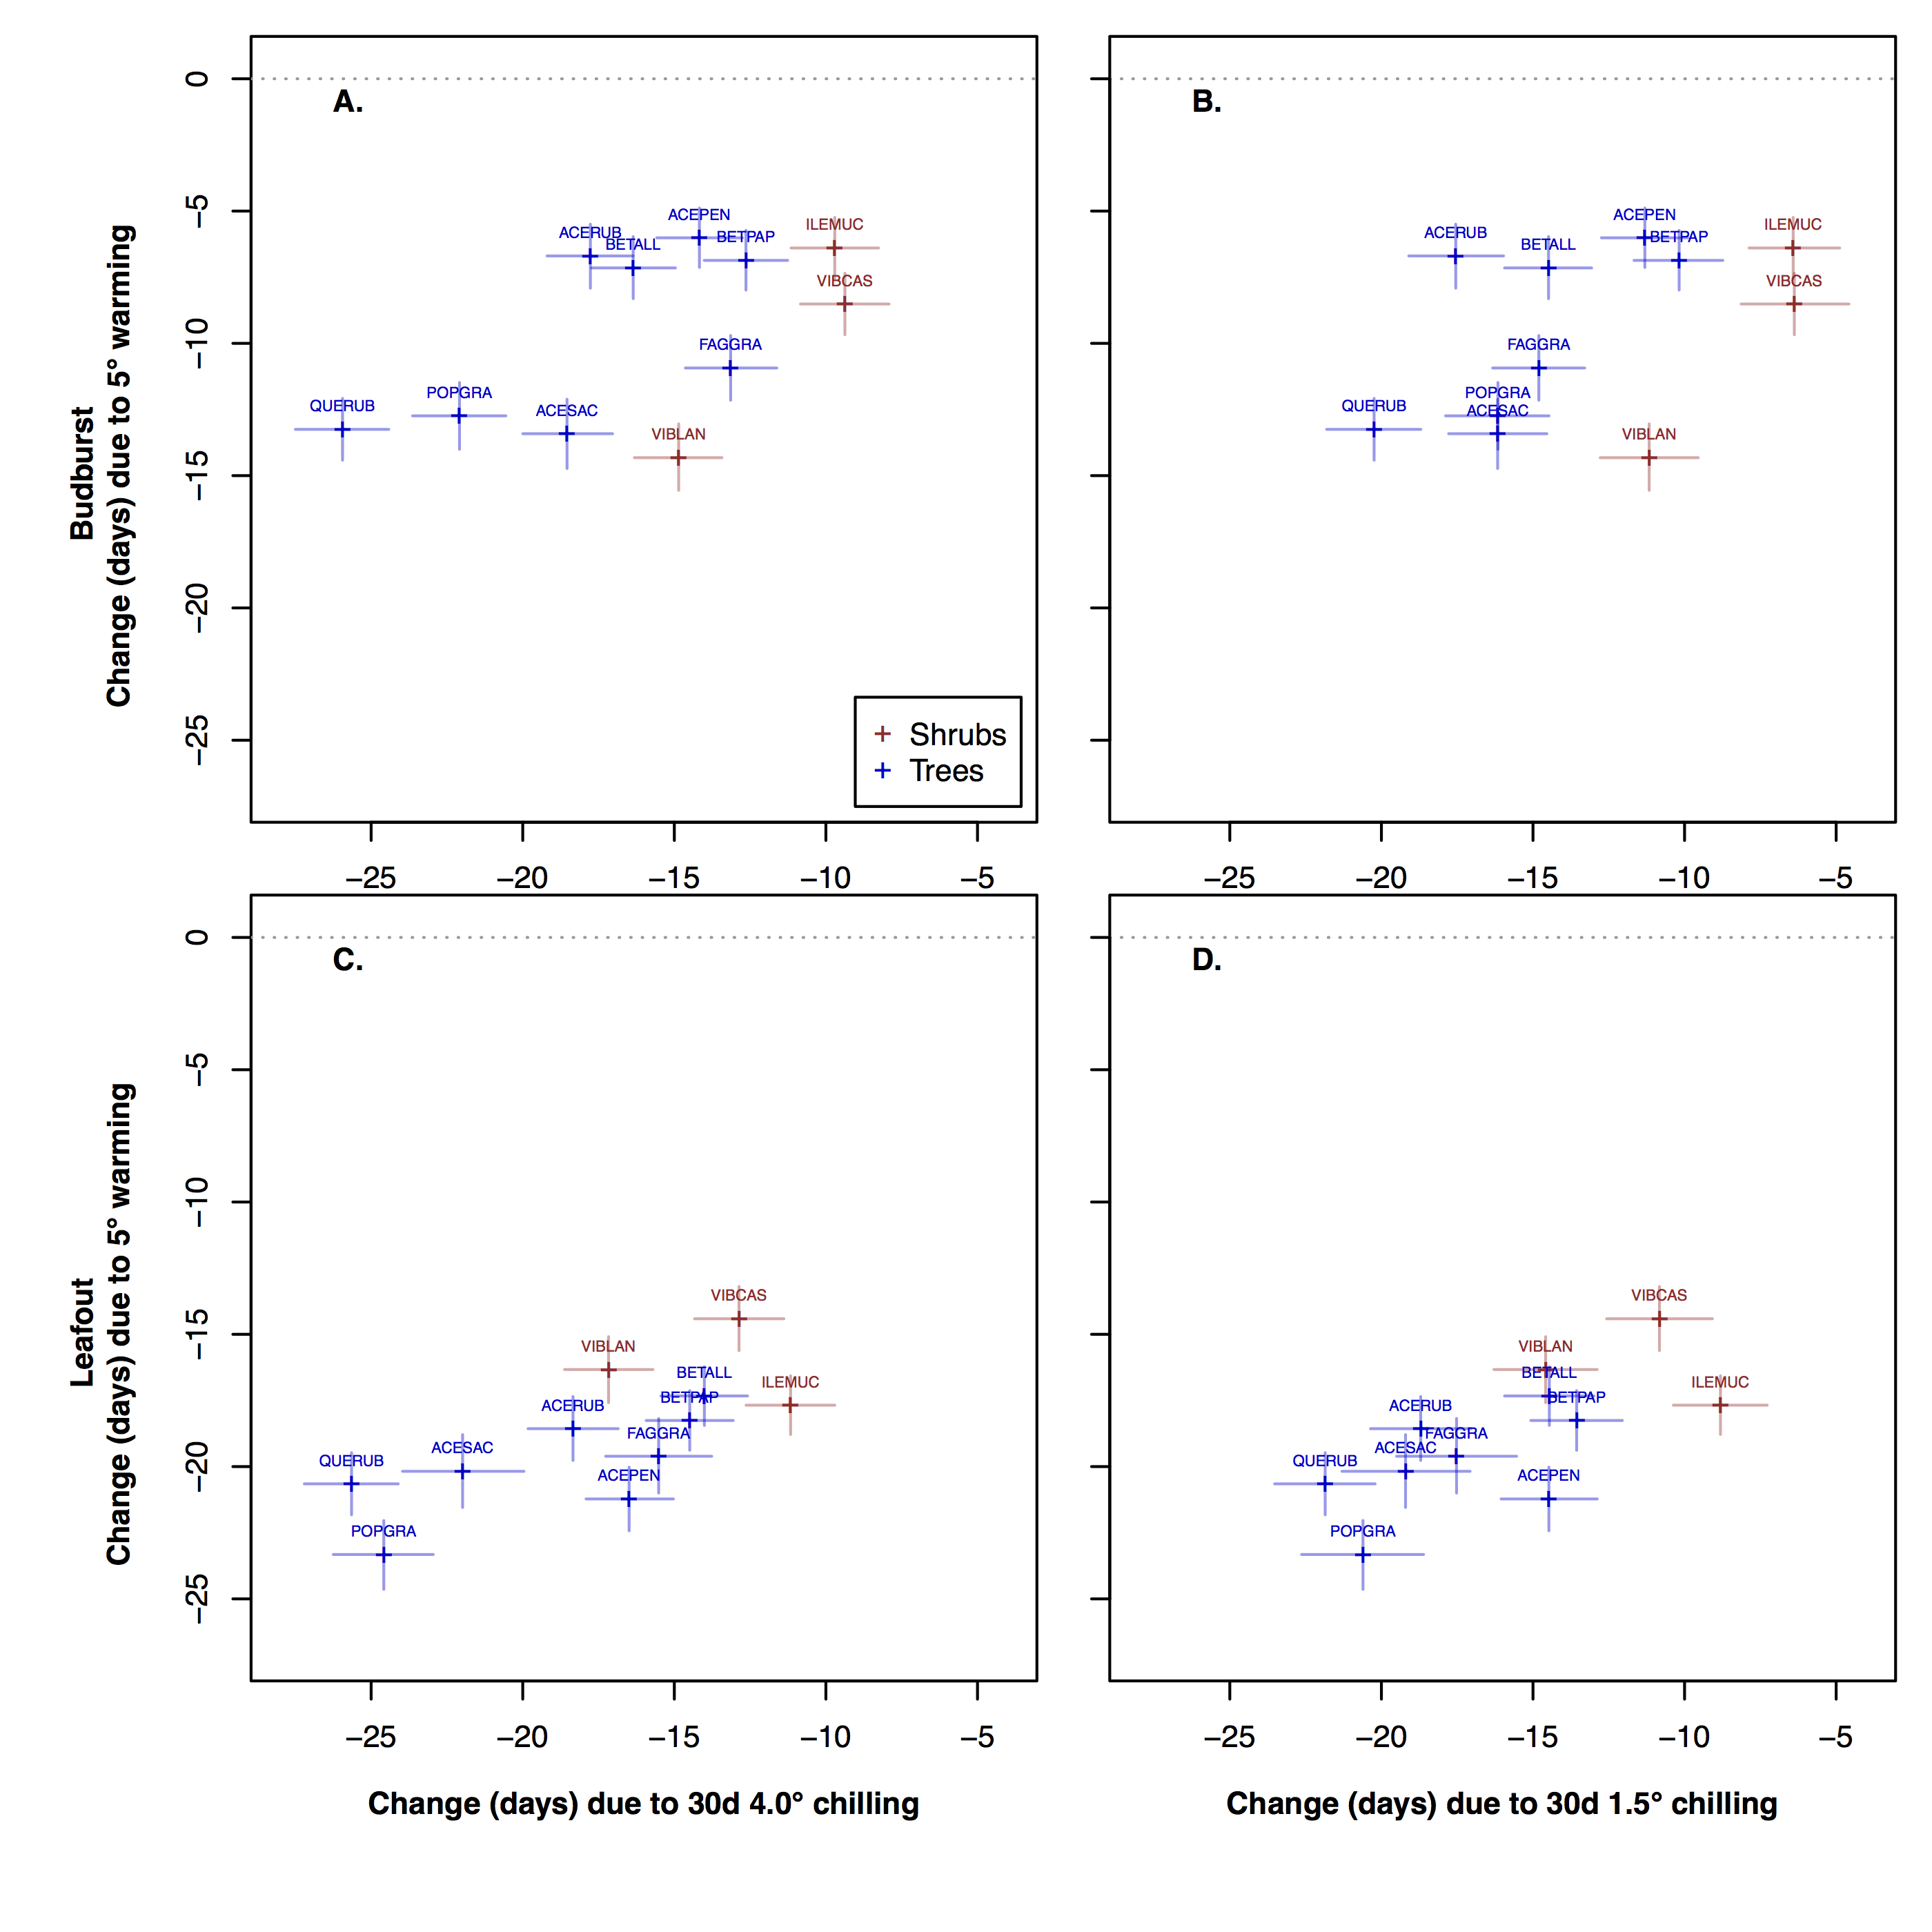
\includegraphics[width=1\textwidth]{FigChill2_4panel.png}
\caption{Effects of temperature and chilling across species (shrub species shown in red, tree species in blue): Similar to Fig. 2 from main text, but showing results side-by-side for the two chilling treatments: 4.0\degree C (left) versus 1.5\degree C (right) as compared to forcing temperature responses (for photoperiod see S8). Crosses and bars show mean and 50\% credible intervals.}
\end{figure}


\begin{figure}
\label{fig:figS7}
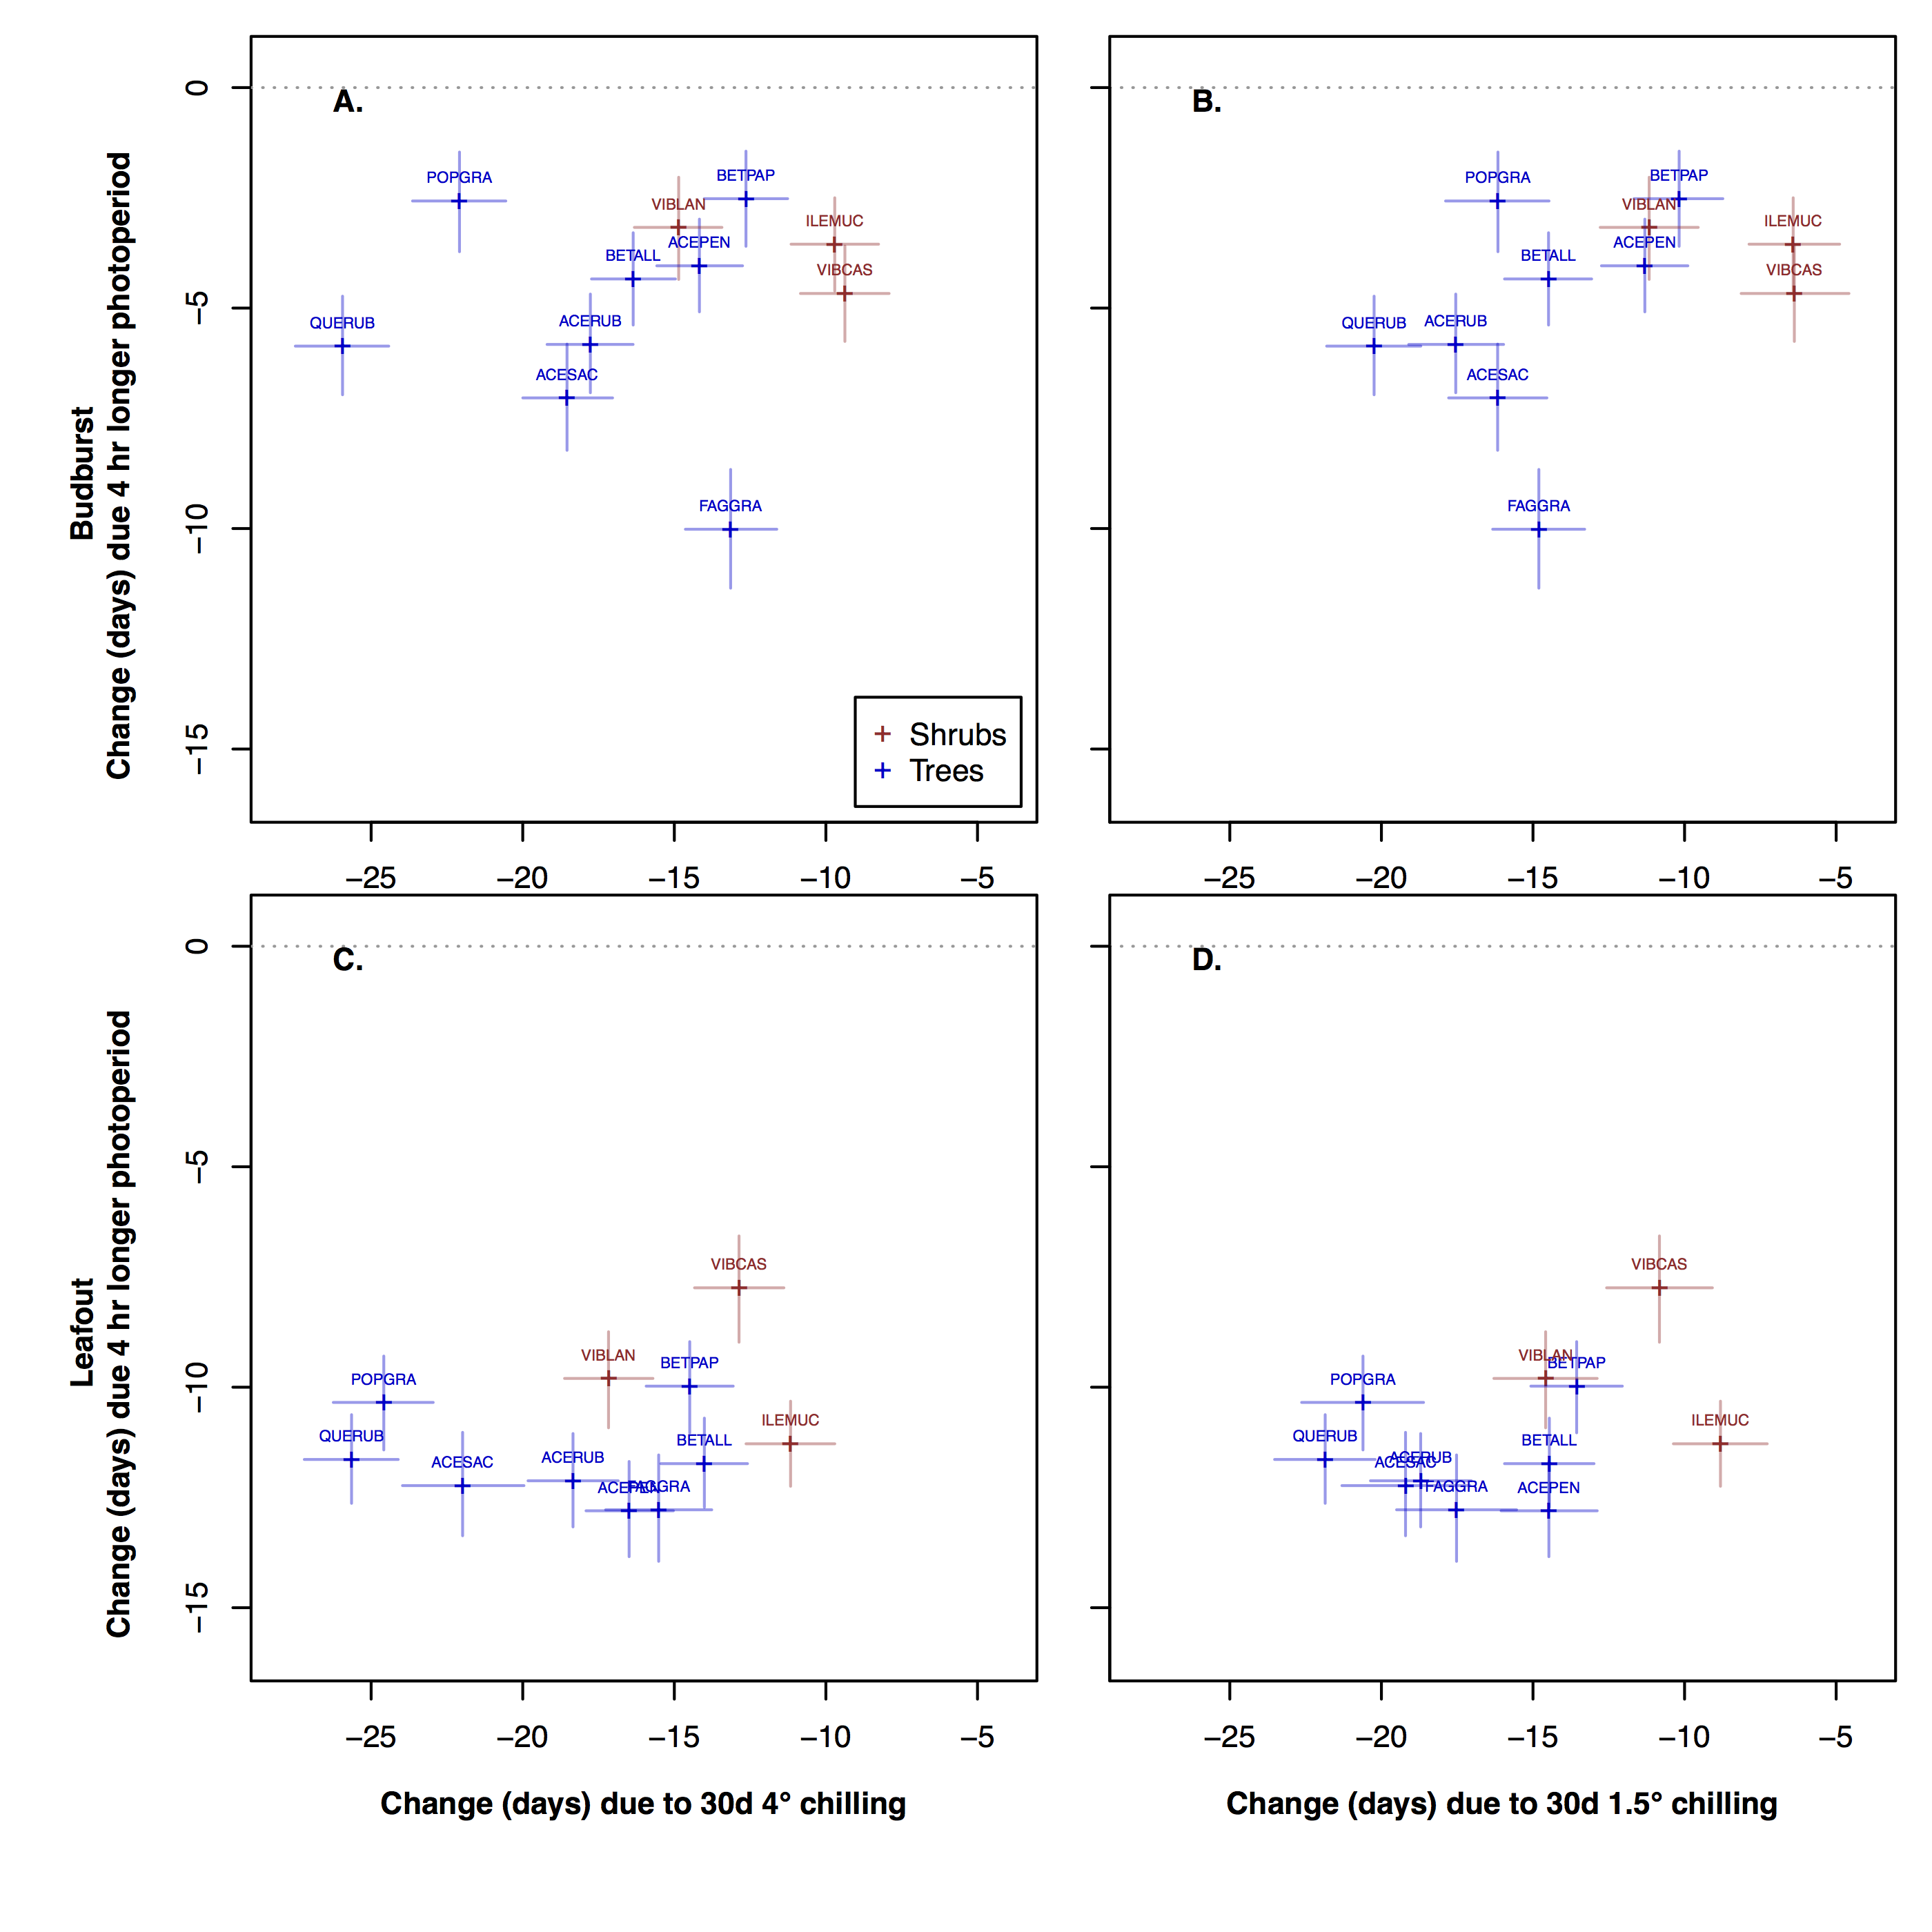
\includegraphics[width=1\textwidth]{FigChillPhoto_4panel.png}
\caption{Effects of photoperiod and chilling across species (shrub species shown in red, tree species in blue): Similar to Fig. 2 from main text, but showing results side-by-side for the two chilling treatments: 4.0\degree C (left) versus 1.5\degree C (right) as compared to photoperiod responses (for forcing temperature see S7). Crosses and bars show mean and 50\% credible intervals.}
\end{figure}

\begin{figure}
\includegraphics[width=1\textwidth]{/Users/Lizzie/Documents/git/projects/treegarden/budchill/analyses/figures/m1and14.png} % see budchill/analyses/budchill_analysis.R 
\caption{Model estimates of effects chilling temperature (1\degree C or 4\degree C) and time (no additional chilling, 16 days additional or 32 days additional chilling) on budburst day (including species-level effects), as assessed from a follow-up experiment conducted in the winter of 2015-2016. Dots and bars show mean and 50\% credible intervals. Note that for this experiment the intercept (not shown: 44.7 days) was the estimate for the 1\degree C treatment.}
\label{fig:figbudchill}
\end{figure}

\end{document}


\noindent\emph{Literature Review} (Note: I am not sure we need this anymore.)

\noindent We conducted a literature review, finding 109 studies which investigated effects of photoperiod, temperature, or their interaction on the timing of bud burst or flowering for woody or semi-woody plants.  No study varied chilling period, photoperiod, and temperature simultaneously across multiple species at multiple sites. Of those studies, eight simultaneously manipulated photoperiod and temperature. \citet{Basler:2014aa} found a negative tradeoff between sensitivity to photoperiod and sensitivity to warming for four species, for example with \emph{Fagus sylvatica} advanced on average in leafout by 12 days in response to experimentally lengthened photoperiod, but only ca. 8 days in response to warmer temperatures, while \emph{Acer pseudoplatanus} advanced in leafout by 17 days in response to warming but essentially had no change in response to photoperiod. The current study expands on this work by including 28 species, across two sites, with addition manipulations of chilling temperature.


%% Trait and HF (O'Keefe) plots
% Used to go before end{document} 
\clearpage

\begin{figure}
\caption{Trait sensitivity based on specific leaf area}
\label{figS5}
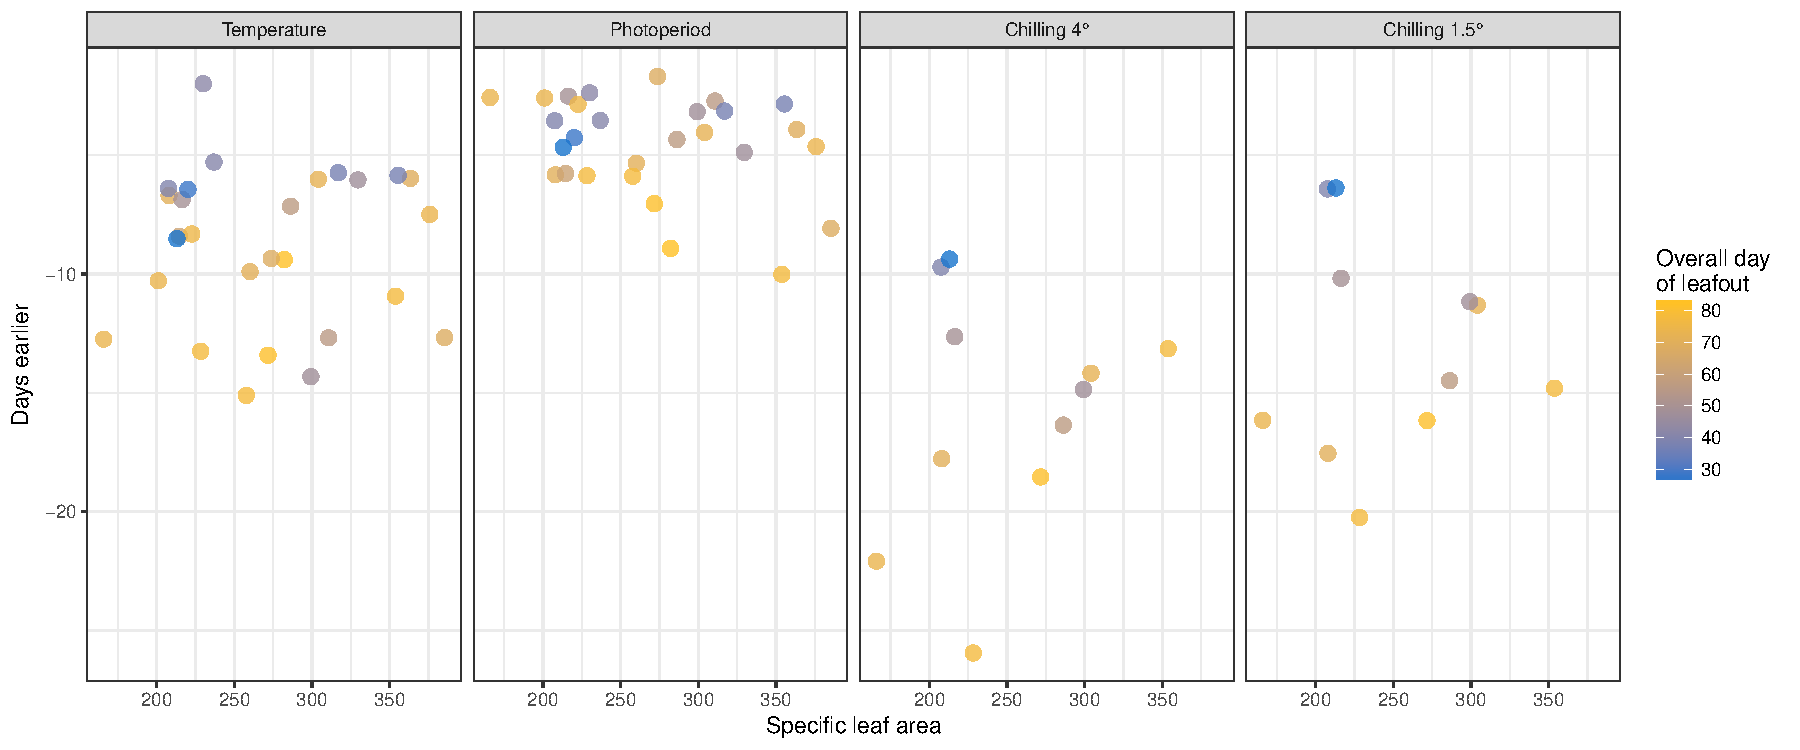
\includegraphics[scale=0.95, page=1]{Traits_vs_sensitivity}
\end{figure}

\begin{figure}
\caption{Trait sensitivity based on stem density}
\label{figS6}
\includegraphics[scale=0.95, page=2]{Traits_vs_sensitivity}
\end{figure}

\begin{figure}
\caption{Trait sensitivity based on \% nitrogen}
\label{figS7}
\includegraphics[scale=0.95, page=3]{Traits_vs_sensitivity}
\end{figure}


\begin{figure}
\caption{Specific leaf area and stem density by trees vs shrubs}
\label{figS8}
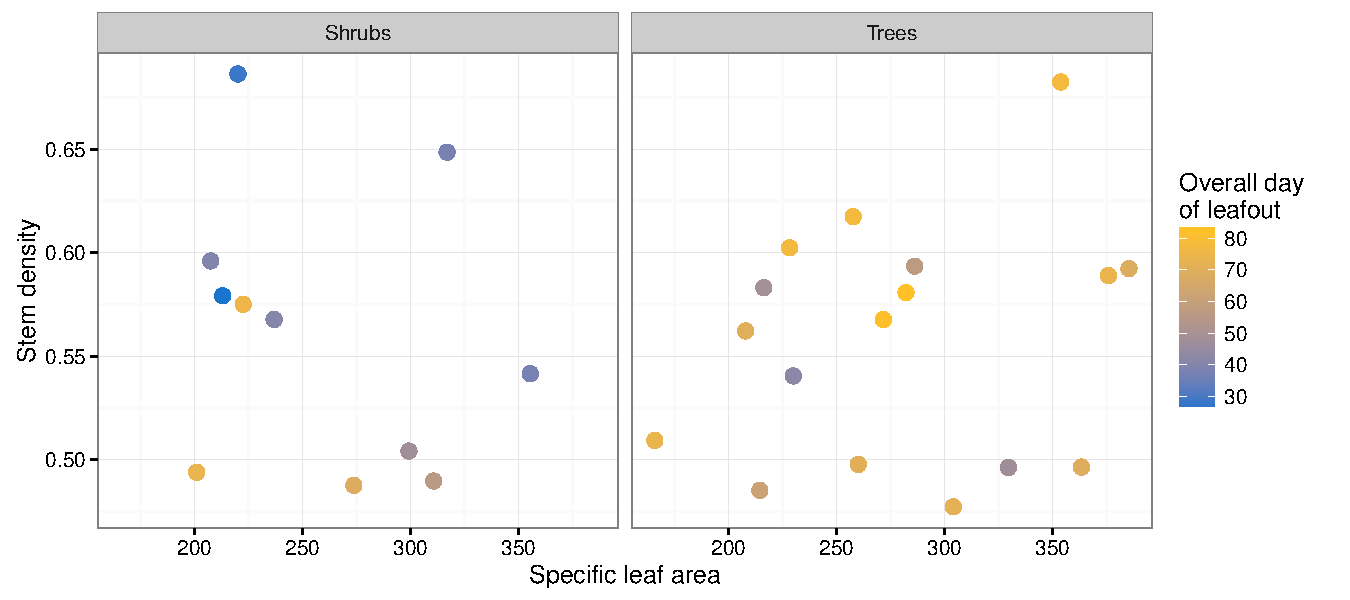
\includegraphics[scale=0.95, page=1]{Tree_shrub_traits}
\end{figure}


\begin{figure}
\caption{Specific leaf area and percent nitrogen by trees vs shrubs}
\label{figS9}
\includegraphics[scale=0.95, page=2]{Tree_shrub_traits}
\end{figure}

\begin{figure}
\caption{Stem density and percent nitrogen by trees vs shrubs}
\label{figS10}
\includegraphics[scale=0.95, page=3]{Tree_shrub_traits}
\end{figure}

\clearpage


\begin{figure}
\caption{Leafout rank order in experimental treatments vs. O'Keefe observations}
\label{figS11}
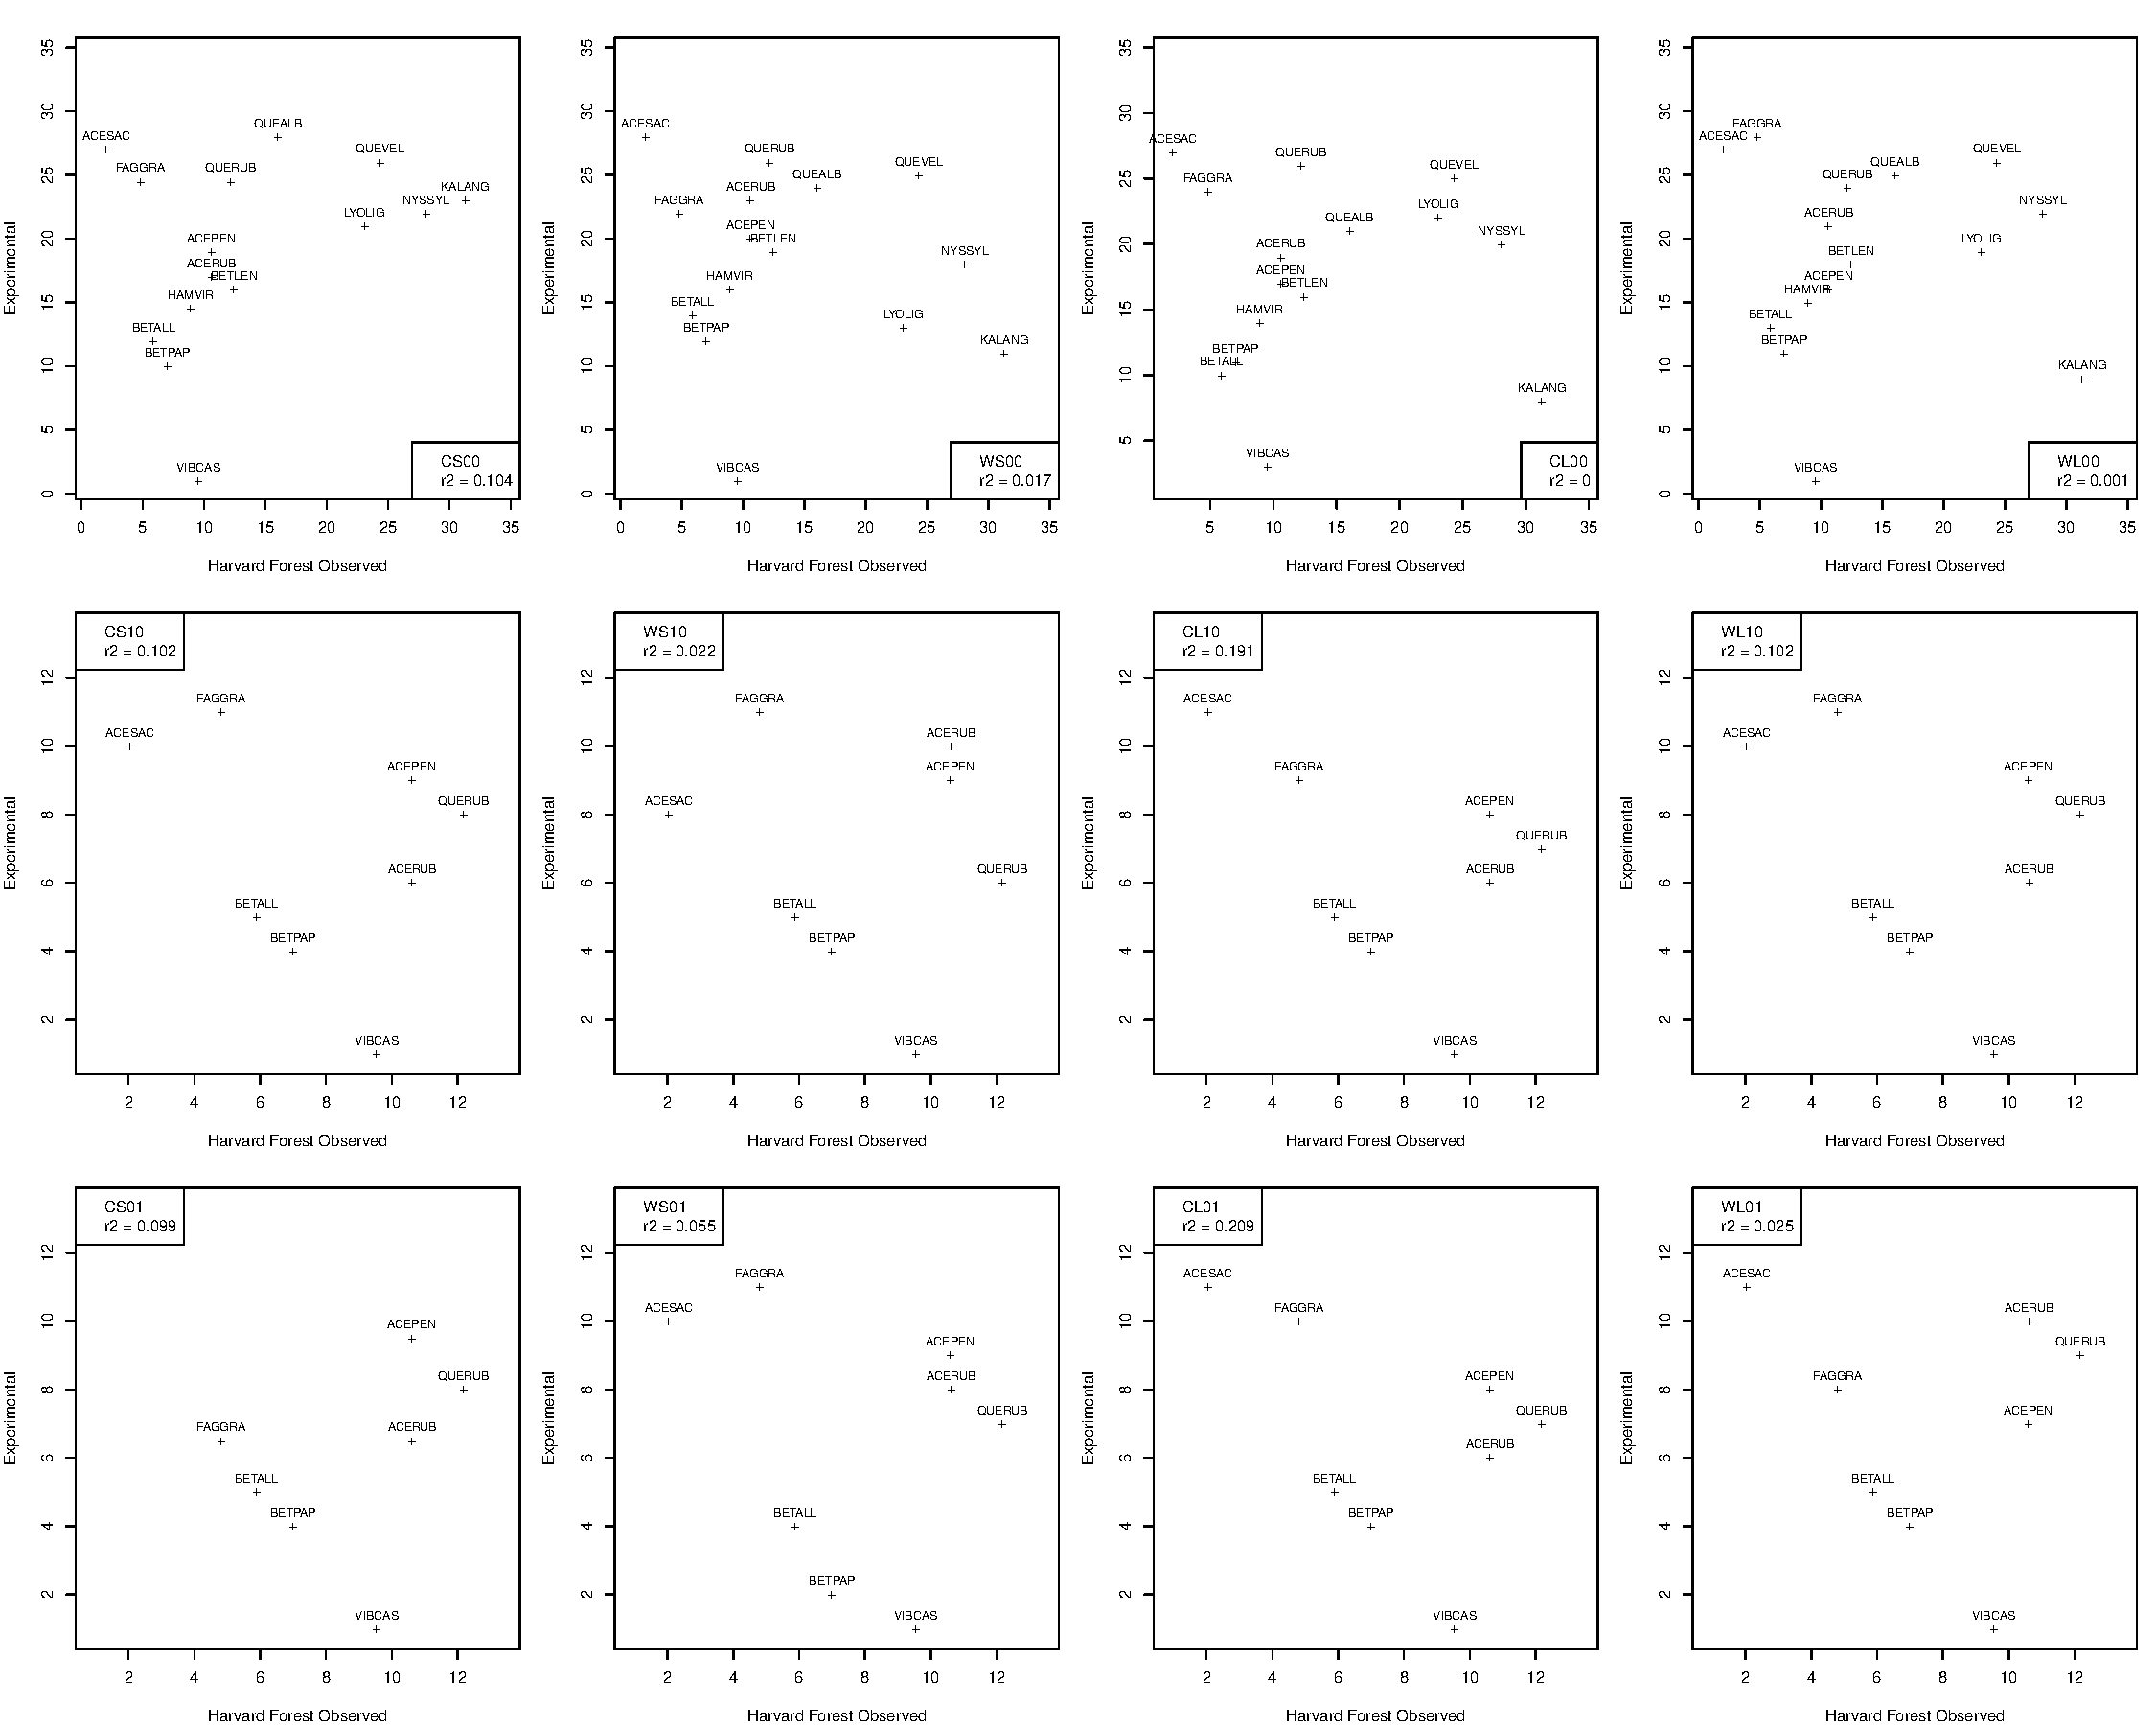
\includegraphics{leafout_exp_obs_corr}
\end{figure}

\begin{figure}
\caption{Leafout day of year in experimental treatments vs. O'Keefe observations}
\label{figS12}
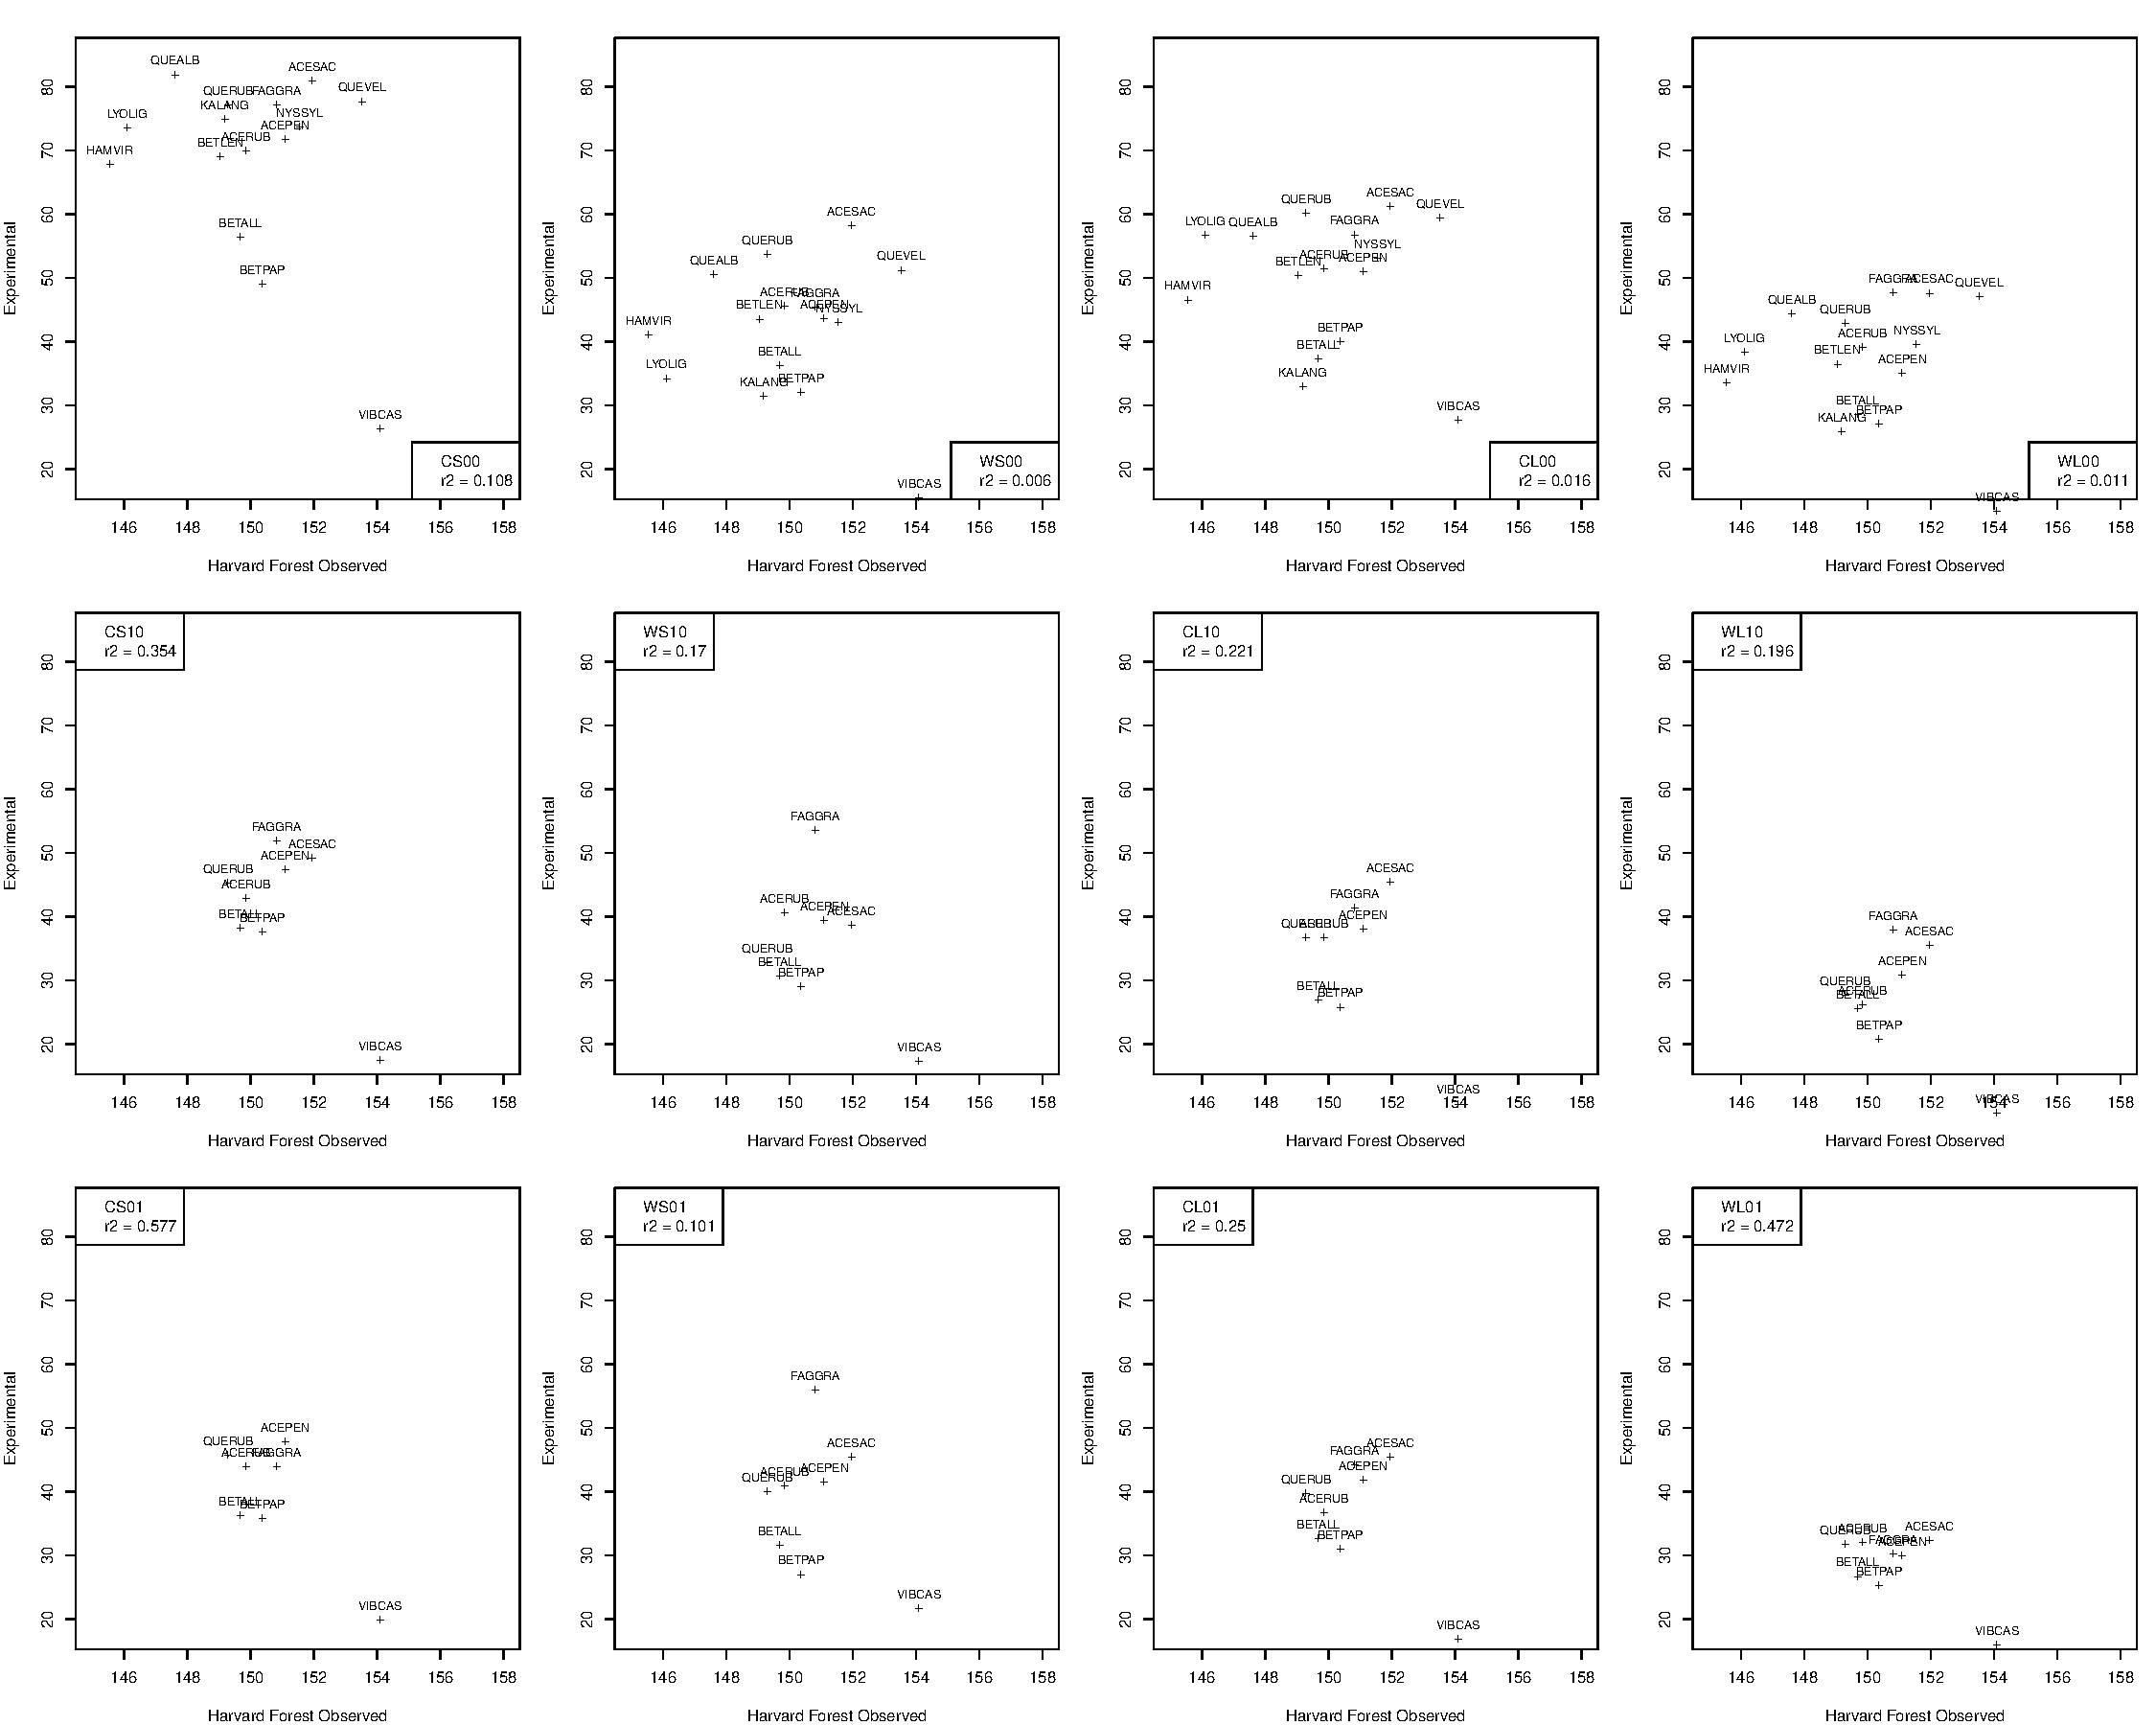
\includegraphics{leafout_exp_obs_corr_day}
\end{figure}

 
